\chapter{Attention Mechanisms and Transformers}
\label{chap:attention_transformers}

\begin{tldr}
Attention mechanisms enable neural networks to dynamically focus on relevant parts of the input. This chapter covers the mathematical foundations of attention (additive, multiplicative, scaled dot-product), self-attention and multi-head attention, the complete Transformer architecture, positional encodings (sinusoidal, learned, RoPE, ALiBi), efficient attention variants (fixed and trainable sparsity, linear attention, FlashAttention 1--3 and Flash-Decoding, MQA/GQA/MLA), and modern design choices (pre-norm, GQA, SwiGLU, and the 2024--26 refinements: QK-norm, interleaved sliding-window attention, large vocabularies). Understanding attention deeply---including computational complexity and memory requirements---is essential for staff-level ML interviews.
\end{tldr}

\section{Attention as a Computational Primitive}
\label{sec:attention_primitive}

\subsection{The Core Intuition}

Attention can be understood as a \textbf{soft dictionary lookup}:

\begin{itemize}
    \item \textbf{Query} ($\vq$): What you're looking for
    \item \textbf{Keys} ($\vk$): What each item ``is'' (index)
    \item \textbf{Values} ($\vv$): What information to retrieve
\end{itemize}

\begin{equation}
\text{output} = \sum_i \underbrace{\text{similarity}(\vq, \vk_i)}_{\text{attention weight}} \cdot \vv_i
\end{equation}

Unlike hard dictionary lookup (exact match), attention computes a weighted combination based on similarity.

\subsection{Mathematical Formulation}

\textbf{General Attention.}
Given query $\vq \in \R^{d_q}$, keys $\mK \in \R^{n \times d_k}$, and values $\mV \in \R^{n \times d_v}$:
\begin{equation}
\text{Attention}(\vq, \mK, \mV) = \sum_{i=1}^{n} \alpha_i \vv_i = \bm{\alpha}^T \mV
\end{equation}
where attention weights $\bm{\alpha} = \softmax(\bm{e})$ and $\bm{e} = [e_1, \ldots, e_n]$ are alignment scores.

The choice of alignment function $e_i = f(\vq, \vk_i)$ defines different attention mechanisms.

%==============================================================================
\section{Types of Attention Mechanisms}
\label{sec:attention_types}
%==============================================================================

\subsection{Additive (Bahdanau) and Multiplicative (Luong) Attention}

The first attention mechanisms came from neural machine translation. \textbf{Additive (Bahdanau) attention} (Bahdanau et al., 2014) scores each query--key pair with a small MLP:
\begin{equation}
e_i = \vv_a^T \tanh(\mW_q \vq + \mW_k \vk_i + \vb)
\end{equation}
\textbf{Multiplicative (Luong) attention} (Luong et al., 2015) replaces the MLP with a bilinear form $e_i = \vq^T \mW_a \vk_i$, or a plain dot product $e_i = \vq^T \vk_i$ when query and key dimensions match.

\textbf{Additive vs.\ multiplicative.} Multiplicative attention is faster in practice because the score computation reduces to a single matrix multiply, which is heavily optimized on GPUs. Additive attention is more expressive for small $d_k$ because the $\tanh$ nonlinearity can learn complex alignment patterns. For large $d_k$ (as in Transformers), the expressivity gap vanishes and the speed advantage of multiplicative attention dominates. This is why scaled dot-product attention became the standard.

\textbf{Local attention precursor.} Luong also proposed a \emph{local} variant that predicts an aligned position $p_t$ and attends only to a window $[p_t - D, p_t + D]$---$O(D)$ per step regardless of source length, and a direct precursor of the sliding-window attention in modern efficient Transformers (Longformer, Mistral).

\textbf{Lineage}: Bahdanau (2014) and Luong (2015) established the attention vocabulary of queries, keys, values, and alignment scores that Vaswani et al.\ (2017) generalized into self-attention and the Transformer. The progression from additive $\to$ multiplicative $\to$ scaled dot-product is a direct lineage.

\subsection{Scaled Dot-Product Attention}

\begin{mathresult}{Scaled Dot-Product Attention}
\begin{equation}
\text{Attention}(\mQ, \mK, \mV) = \softmax\left(\frac{\mQ\mK^T}{\sqrt{d_k}}\right)\mV
\end{equation}
\end{mathresult}

This is the attention mechanism used in Transformers.

\subsubsection{Why Scale by $\sqrt{d_k}$?}

Without scaling, dot products grow with dimension $d$ (their variance equals $d$). This pushes softmax into saturation where gradients vanish. Dividing by $\sqrt{d_k}$ restores unit variance and keeps gradients healthy.

\begin{figure}[H]
\centering
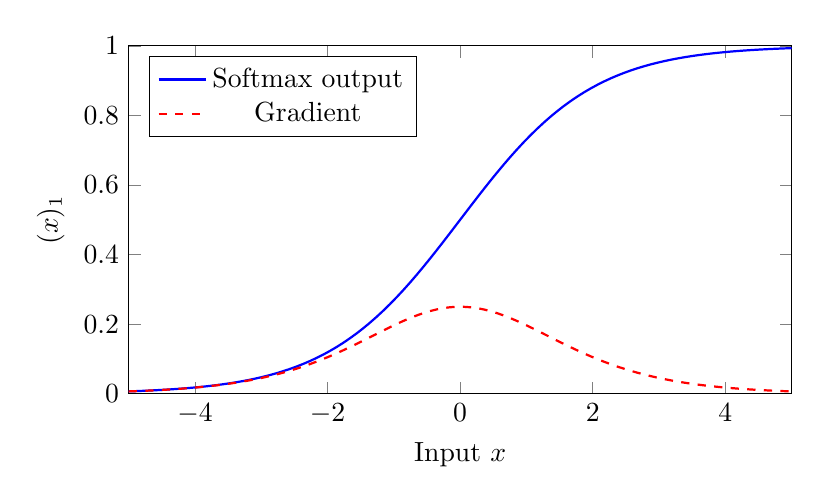
\begin{tikzpicture}
    \begin{axis}[
        xlabel={Input $x$},
        ylabel={$\softmax(x)_1$},
        xmin=-5, xmax=5,
        ymin=0, ymax=1,
        legend pos=north west,
        width=10cm,
        height=6cm
    ]
    % For 2 classes, softmax(x) vs softmax(-x)
    \addplot[domain=-5:5, samples=100, thick, blue] {exp(x)/(exp(x)+exp(0))};
    \addlegendentry{Softmax output}

    % Gradient visualization
    \addplot[domain=-5:5, samples=100, thick, red, dashed] {exp(x)/(exp(x)+exp(0)) * (1 - exp(x)/(exp(x)+exp(0)))};
    \addlegendentry{Gradient}
    \end{axis}
\end{tikzpicture}
\caption{Softmax output and gradient. Large inputs cause saturation where gradients vanish.}
\label{fig:softmax_saturation}
\end{figure}

%==============================================================================
\section{Self-Attention}
\label{sec:self_attention}
%==============================================================================

\subsection{Definition}

In self-attention, queries, keys, and values all come from the same sequence:

\begin{mathresult}{Self-Attention}
Given input sequence $\mX \in \R^{n \times d}$:
\begin{align}
\mQ &= \mX \mW^Q, \quad \mK = \mX \mW^K, \quad \mV = \mX \mW^V \\
\text{SelfAttention}(\mX) &= \softmax\left(\frac{\mQ\mK^T}{\sqrt{d_k}}\right)\mV
\end{align}
where $\mW^Q, \mW^K \in \R^{d \times d_k}$ and $\mW^V \in \R^{d \times d_v}$.
\end{mathresult}

\subsection{What Self-Attention Computes}

For each position $i$:
\begin{equation}
\vy_i = \sum_{j=1}^n \alpha_{ij} \vv_j
\end{equation}
where $\alpha_{ij} = \softmax_j\left(\frac{\vq_i^T \vk_j}{\sqrt{d_k}}\right)$.

\textbf{Interpretation}: Position $i$'s output is a weighted combination of all positions' values, weighted by query-key similarity.

\subsection{Computational Complexity}

\textbf{Self-Attention Complexity.}
For sequence length $n$ and dimension $d$:
\begin{itemize}
    \item \textbf{Time}: $O(n^2 d)$ for attention scores + $O(n^2 d)$ for weighted sum = $O(n^2 d)$
    \item \textbf{Memory}: $O(n^2)$ for attention matrix + $O(nd)$ for embeddings
\end{itemize}

The $O(n^2)$ complexity is the fundamental limitation for long sequences.

\subsection{Properties of Self-Attention}

\begin{enumerate}
    \item \textbf{Permutation equivariant}: $\text{SelfAttn}(\pi(\mX)) = \pi(\text{SelfAttn}(\mX))$
    \begin{itemize}
        \item The operation itself doesn't know position
        \item Position must be injected via positional encodings
    \end{itemize}

    \item \textbf{Global receptive field}: Every position can attend to every other position from layer 1
    \begin{itemize}
        \item Unlike CNNs (local) or RNNs (sequential)
        \item Enables modeling long-range dependencies
    \end{itemize}

    \item \textbf{Dynamic}: Attention pattern depends on input content
    \begin{itemize}
        \item Unlike convolution with fixed kernel
        \item Can learn different patterns for different inputs
    \end{itemize}
\end{enumerate}

%==============================================================================
\section{Multi-Head Attention}
\label{sec:multi_head}
%==============================================================================

\subsection{Motivation}

Single attention head learns one type of relationship. Multiple heads learn diverse patterns:
\begin{itemize}
    \item Some heads focus on local context
    \item Some heads capture long-range dependencies
    \item Different heads for different syntactic/semantic roles
\end{itemize}

\subsection{Mathematical Formulation}

\begin{mathresult}{Multi-Head Attention}
\begin{align}
\text{MultiHead}(\mQ, \mK, \mV) &= \text{Concat}(\text{head}_1, \ldots, \text{head}_h)\mW^O \\
\text{head}_i &= \text{Attention}(\mQ\mW_i^Q, \mK\mW_i^K, \mV\mW_i^V)
\end{align}
where $\mW_i^Q, \mW_i^K \in \R^{d \times d_k}$, $\mW_i^V \in \R^{d \times d_v}$, $\mW^O \in \R^{hd_v \times d}$, and typically $d_k = d_v = d/h$.
\end{mathresult}

\subsection{Implementation Detail}

\textbf{Efficient computation}: Instead of $h$ separate attention operations:
\begin{enumerate}
    \item Project $\mQ, \mK, \mV$ to shape $(n, h, d_k)$
    \item Transpose to $(h, n, d_k)$ for batched matrix multiplication
    \item Compute all heads in parallel
    \item Concatenate and project
\end{enumerate}

\subsection{Parameter Count}

For model dimension $d$ with $h$ heads:
\begin{align}
\mW^Q, \mW^K, \mW^V &: 3 \times d \times d = 3d^2 \\
\mW^O &: d \times d = d^2 \\
\text{Total} &: 4d^2
\end{align}

\subsection{What Different Heads Learn}

Empirical observations:
\begin{itemize}
    \item \textbf{Positional heads}: Attend to fixed relative positions
    \item \textbf{Syntactic heads}: Subject-verb, modifier-noun relationships
    \item \textbf{Rare word heads}: Attend to infrequent tokens
    \item \textbf{Delimiter heads}: Attend to [SEP], periods
    \item \textbf{Previous/next token heads}: Local context
\end{itemize}

\begin{keyinsight}[Induction Heads: The Mechanistic View]
Mechanistic interpretability decomposes a head into two circuits: the \textbf{QK circuit} decides \textit{where} to attend, and the \textbf{OV circuit} decides \textit{what} information is copied to the output once attention lands there. The best-understood composite mechanism is the \textbf{induction head}: given a repeated pattern $[A][B] \ldots [A]$, it attends from the second $[A]$ to the token \textit{after} the previous occurrence of $[A]$ and copies it---predicting $[B]$. It works via two-layer composition: an earlier ``previous-token head'' writes each token's predecessor into the residual stream, so the induction head's QK circuit can match ``current token $=$ token that preceded you,'' and its OV circuit copies the matched token forward. Olsson et al.\ (2022) showed induction heads form abruptly during a phase change early in training, coincident with the emergence of in-context learning---the leading mechanistic account of why Transformers can learn from their prompt. The modern answer to ``what do attention heads do'' is this circuit-level story, not BERT-era probing taxonomies.
\end{keyinsight}

%==============================================================================
\section{The Transformer Architecture}
\label{sec:transformer_arch}
%==============================================================================

\subsection{Overview}

\begin{figure}[H]
\centering
\begin{tikzpicture}[
    node distance=0.7cm,
    box/.style={rectangle, draw, minimum width=3cm, minimum height=0.7cm, rounded corners},
    block/.style={box, fill=lightblue},
    norm/.style={box, fill=lightyellow, minimum width=2.5cm},
    ffn/.style={box, fill=lightgreen},
    input/.style={box, fill=lightgray},
    attention/.style={box, fill=orange!30}
]
    % Input
    \node[input] (input) {Input Embeddings + Position};

    % Encoder block
    \node[attention, above=0.5cm of input] (attn1) {Multi-Head Self-Attention};
    \node[norm, above=0.3cm of attn1] (norm1) {Add \& LayerNorm};
    \node[ffn, above=0.3cm of norm1] (ffn1) {Feed-Forward Network};
    \node[norm, above=0.3cm of ffn1] (norm2) {Add \& LayerNorm};

    % Block indicator
    \draw[thick, decorate, decoration={brace, amplitude=10pt, raise=5pt}]
        ($(attn1.south west)+(-0.5,0)$) -- ($(norm2.north west)+(-0.5,0)$)
        node[midway, left=15pt, font=\small] {$\times N$};

    % Output
    \node[above=0.5cm of norm2] (output) {To next layer / Output};

    % Residual connections
    \draw[->] (input) -- (attn1);
    \draw[->] (attn1) -- (norm1);
    \draw[->] (norm1) -- (ffn1);
    \draw[->] (ffn1) -- (norm2);
    \draw[->] (norm2) -- (output);

    % Residual arrows
    \draw[->, dashed, gray] (input.east) -- ++(0.8,0) |- (norm1.east);
    \draw[->, dashed, gray] (norm1.east) -- ++(0.5,0) |- (norm2.east);

\end{tikzpicture}
\caption{Single Transformer encoder block (post-norm variant).}
\label{fig:transformer_block}
\end{figure}

\subsection{Encoder Block}

Each encoder block consists of:

\begin{enumerate}
    \item \textbf{Multi-Head Self-Attention}
    \begin{equation}
    \tilde{\mH} = \text{MultiHeadAttention}(\mH, \mH, \mH)
    \end{equation}

    \item \textbf{Residual Connection + Layer Normalization}
    \begin{equation}
    \mH' = \text{LayerNorm}(\mH + \tilde{\mH})
    \end{equation}

    \item \textbf{Position-wise Feed-Forward Network}
    \begin{equation}
    \text{FFN}(\vx) = \mW_2 \cdot \sigma(\mW_1 \vx + \vb_1) + \vb_2
    \end{equation}
    Typically with expansion factor 4: $\mW_1 \in \R^{d \times 4d}$, $\mW_2 \in \R^{4d \times d}$.

    \item \textbf{Another Residual + LayerNorm}
    \begin{equation}
    \mH'' = \text{LayerNorm}(\mH' + \text{FFN}(\mH'))
    \end{equation}
\end{enumerate}

\subsection{Decoder Block}

Decoder adds:
\begin{enumerate}
    \item \textbf{Masked Self-Attention}: Prevents attending to future positions
    \item \textbf{Cross-Attention}: Attends to encoder outputs
\end{enumerate}

\begin{mathresult}{Causal Mask}
\begin{equation}
M_{ij} = \begin{cases}
0 & \text{if } j \leq i \\
-\infty & \text{if } j > i
\end{cases}
\end{equation}
Applied as: $\softmax\left(\frac{\mQ\mK^T}{\sqrt{d_k}} + \mathbf{M}\right)$
\end{mathresult}

\subsection{Pre-Norm vs Post-Norm}

\textbf{Post-Norm (Original Transformer)}:
\begin{equation}
\mH' = \text{LayerNorm}(\mH + \text{SubLayer}(\mH))
\end{equation}

\textbf{Pre-Norm (Modern Standard)}:
\begin{equation}
\mH' = \mH + \text{SubLayer}(\text{LayerNorm}(\mH))
\end{equation}

\begin{table}[H]
\centering
\caption{Pre-Norm vs Post-Norm comparison}
\begin{tabularx}{\textwidth}{lXX}
\toprule
\textbf{Aspect} & \textbf{Post-Norm} & \textbf{Pre-Norm} \\
\midrule
Gradient flow & Through LayerNorm & Direct residual path \\
Training stability & Needs warmup & More stable \\
Final performance & Slightly better (when stable) & Very close \\
Modern usage & Rare & Standard (GPT, LLaMA, etc.) \\
\bottomrule
\end{tabularx}
\end{table}

\begin{keyinsight}[Why Pre-Norm Stabilizes Training]
Pre-norm is more stable because the residual path doesn't pass through normalization:
\begin{equation}
\frac{\partial \loss}{\partial \mH} = \frac{\partial \loss}{\partial \mH'} \cdot \left(\mI + \frac{\partial \text{SubLayer}}{\partial \mH}\right)
\end{equation}
The identity term $\mI$ ensures gradient always flows, preventing vanishing gradients.
\end{keyinsight}

%==============================================================================
\section{Positional Encodings}
\label{sec:positional}
%==============================================================================

\subsection{Why Position Information is Needed}

Self-attention is \textbf{permutation equivariant}:
\begin{equation}
\text{SelfAttn}(\pi(\mX)) = \pi(\text{SelfAttn}(\mX))
\end{equation}

Without positional information, ``The cat sat on the mat'' and ``mat the on sat cat The'' produce the same output!

\subsection{Sinusoidal Positional Encoding}

\begin{mathresult}{Sinusoidal Encoding (Original Transformer)}
\begin{align}
PE_{(pos, 2i)} &= \sin\left(\frac{pos}{10000^{2i/d}}\right) \\
PE_{(pos, 2i+1)} &= \cos\left(\frac{pos}{10000^{2i/d}}\right)
\end{align}
\end{mathresult}

\textbf{Properties}:
\begin{itemize}
    \item Deterministic, no learned parameters
    \item Each dimension has different frequency
    \item Can extrapolate to longer sequences than seen in training
\end{itemize}

\textbf{Why it enables relative position}:
For any fixed offset $k$:
\begin{equation}
PE_{pos+k} = f_k(PE_{pos})
\end{equation}
where $f_k$ is a linear transformation (rotation matrix). This allows the model to learn to attend to relative positions.

\subsection{Learned Positional Embeddings}

\textbf{Learned Positional Embedding.} Instead of using a fixed function of position, maintain a trainable embedding matrix $\mathbf{P} \in \R^{L_{\max} \times d_{\text{model}}}$ where each row corresponds to a position index. The position encoding for token at position $t$ is simply:

\begin{equation}
\mE_{pos} \in \R^{L_{max} \times d}, \quad \text{PE}(t) = \mathbf{P}[t, :]
\end{equation}

This embedding is added to the token embedding exactly as with sinusoidal encodings: $\vx_t = \text{TokenEmbed}(w_t) + \mathbf{P}[t, :]$. The matrix $\mathbf{P}$ is initialized randomly and learned end-to-end via backpropagation.

\textbf{Key difference from sinusoidal}: Sinusoidal encodings have a built-in inductive bias for relative positions (the linear-transformation property between positions), while learned embeddings treat each position as an independent embedding with no structural relationship. This means learned PE must discover positional patterns purely from data.

\textbf{Used in}: BERT (max 512), GPT-2 (max 1024), early GPT-3

\begin{warningbox}
Learned positional embeddings impose a hard sequence length ceiling at $L_{\max}$. At inference time, any position $t \geq L_{\max}$ has no trained embedding---the model either crashes or produces garbage. This is not a soft degradation; it is a cliff. This is the primary reason the field moved away from learned PE for generative models that need flexible context windows.
\end{warningbox}

\textbf{Positional Encoding Comparison} --- when each strategy fits:

\begin{itemize}
    \item \textbf{Sinusoidal (Vaswani et al., 2017).} Fixed, no learned parameters, theoretically extrapolates but empirically degrades. Useful as a simple baseline and in settings where you want deterministic encodings.
    \item \textbf{Learned (BERT, GPT-2).} Slightly higher accuracy than sinusoidal within training lengths, but zero extrapolation ability. Suitable for fixed-length encoder tasks (classification, NLI) where $L_{\max}$ is known in advance.
    \item \textbf{RoPE (Su et al., 2021).} Encodes relative position via rotation matrices applied to Q/K. Naturally captures relative distance, and extrapolates beyond training length via NTK-aware scaling or YaRN. Default choice for modern LLMs (LLaMA, Mistral, Qwen).
    \item \textbf{ALiBi (Press et al., 2022).} Adds a static linear bias $-m \cdot |i - j|$ directly to attention scores (no change to embeddings). Zero extra parameters, strong extrapolation, but slightly less expressive than RoPE. Used in BLOOM and MPT.
\end{itemize}

\textbf{Why RoPE won.} Most modern autoregressive models need to (a) handle relative positions for generalization and (b) extrapolate to longer sequences at inference via techniques like NTK-aware scaling or dynamic NTK. Learned PE fails both requirements. Sinusoidal PE handles (a) in theory but degrades in practice. RoPE achieves both cleanly, which is why it became the de facto standard from LLaMA onward.

\subsection{Relative Positional Encodings}

\subsubsection{Shaw et al. Relative Attention}

Add relative position embeddings to keys:
\begin{equation}
e_{ij} = \frac{(\vx_i \mW^Q)(\vx_j \mW^K + \va_{j-i}^K)^T}{\sqrt{d_k}}
\end{equation}

Optionally also to values:
\begin{equation}
\vz_i = \sum_j \alpha_{ij}(\vx_j \mW^V + \va_{j-i}^V)
\end{equation}

\textbf{Used in}: Transformer-XL, T5

\subsection{Rotary Position Embedding (RoPE)}

\begin{mathresult}{RoPE}
Encode position by rotating query and key vectors:
\begin{equation}
f(\vx, m) = \mR_m \vx
\end{equation}
where $\mR_m$ is a rotation matrix dependent on position $m$.
\end{mathresult}

For 2D subspaces:
\begin{equation}
\mR_m = \begin{pmatrix}
\cos(m\theta_1) & -\sin(m\theta_1) & & \\
\sin(m\theta_1) & \cos(m\theta_1) & & \\
& & \ddots & \\
& & & \cos(m\theta_{d/2}) & -\sin(m\theta_{d/2}) \\
& & & \sin(m\theta_{d/2}) & \cos(m\theta_{d/2})
\end{pmatrix}
\end{equation}

\textbf{Key property}: Relative position naturally encoded:
\begin{equation}
(\mR_m \vq)^T (\mR_n \vk) = \vq^T \mR_m^T \mR_n \vk = \vq^T \mR_{n-m} \vk
\end{equation}

\textbf{Used in}: LLaMA, Mistral, most modern open LLMs

\textbf{Advantages}:
\begin{itemize}
    \item No explicit position embeddings
    \item Naturally encodes relative positions
    \item Good extrapolation
    \item Efficient implementation
\end{itemize}

\begin{warningbox}
Positional encoding extrapolation is not free. A model trained with 4K context won't magically work at 32K just because it uses RoPE or ALiBi. You still need position interpolation, continued pre-training, or progressive extension to reliably handle longer contexts.
\end{warningbox}

\subsection{ALiBi (Attention with Linear Biases)}

\begin{mathresult}{ALiBi}
Add linear bias based on distance:
\begin{equation}
\text{softmax}\left(\frac{\vq_i^T \vk_j}{\sqrt{d_k}} - m \cdot |i - j|\right)
\end{equation}
where $m$ is a head-specific slope.
\end{mathresult}

\textbf{Properties}:
\begin{itemize}
    \item No position embeddings at all
    \item Linear penalty for distance
    \item Excellent length extrapolation
    \item Different heads have different ``attention spans''
\end{itemize}

\textbf{Used in}: BLOOM, MPT

\subsection{Positional Encoding Comparison}

\begin{table}[H]
\centering
\caption{Positional encoding comparison}
\begin{tabularx}{\textwidth}{lXXXX}
\toprule
\textbf{Encoding} & \textbf{Parameters} & \textbf{Extrapolation} & \textbf{Relative} & \textbf{Used In} \\
\midrule
Sinusoidal & None & Degrades empirically & Implicit & Original Transformer \\
Learned & $L \times d$ & Poor & No & BERT, GPT-2 \\
Relative (Shaw) & $O(Ld)$ & Moderate & Explicit & T5, XL \\
RoPE & None & Good & Implicit & LLaMA, Mistral \\
ALiBi & $h$ scalars & Excellent & Implicit & BLOOM, MPT \\
\bottomrule
\end{tabularx}
\end{table}

%==============================================================================
\section{Efficient Attention Variants}
\label{sec:efficient_attention}
%==============================================================================

\subsection{The Efficiency Challenge}

Standard attention: $O(n^2)$ time and memory

\begin{table}[H]
\centering
\caption{Memory for a single $n \times n$ attention matrix (per head, per layer, batch size 1) at different sequence lengths}
\begin{tabular}{lrrr}
\toprule
\textbf{Sequence Length} & \textbf{Attention Matrix} & \textbf{At FP16} & \textbf{At FP32} \\
\midrule
512 & 262K elements & 0.5 MB & 1 MB \\
2,048 & 4.2M elements & 8 MB & 16 MB \\
8,192 & 67M elements & 128 MB & 256 MB \\
32,768 & 1.07B elements & 2 GB & 4 GB \\
131,072 & 17B elements & 32 GB & 64 GB \\
\bottomrule
\end{tabular}
\end{table}

Note these figures are for a \emph{single} head's matrix: naive (pre-Flash-Attention) training materializes one per head, per layer, per batch element, so real memory is $h \times b$ times larger---at 32K with $h=32$ heads that is $\sim$64 GB \emph{per layer} in FP16, which is why avoiding materialization matters so much.

\subsection{Sparse Attention Patterns}

\subsubsection{Local/Sliding Window Attention}

Each position attends only to a window of $w$ neighbors:
\begin{equation}
\alpha_{ij} = 0 \text{ if } |i - j| > w/2
\end{equation}

\textbf{Complexity}: $O(nw)$

\textbf{Used in}: Longformer (with global tokens), Mistral

\subsubsection{Dilated Attention}

Attend to positions at fixed intervals, similar to dilated convolutions.

\subsubsection{Global + Local (Longformer/BigBird)}

\begin{itemize}
    \item Most positions: Local attention (window)
    \item Special tokens (CLS, etc.): Global attention to all positions
\end{itemize}

\begin{figure}[H]
\centering
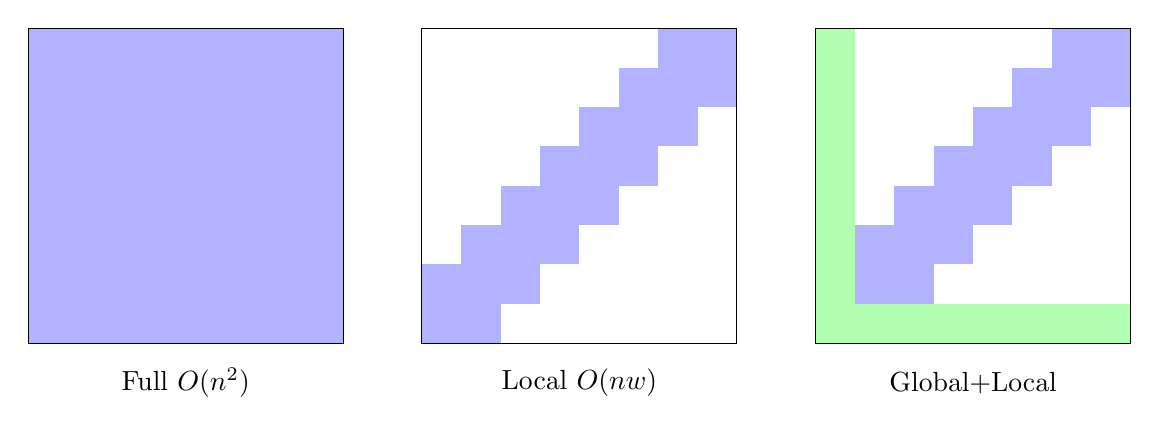
\begin{tikzpicture}[scale=0.5]
    % Full attention
    \begin{scope}[shift={(0,0)}]
        \fill[blue!30] (0,0) rectangle (8,8);
        \draw (0,0) rectangle (8,8);
        \node at (4, -1) {Full $O(n^2)$};
    \end{scope}

    % Local attention
    \begin{scope}[shift={(10,0)}]
        \foreach \i in {0,...,7} {
            \fill[blue!30] ({max(0,\i-1)}, \i) rectangle ({min(8,\i+2)}, {\i+1});
        }
        \draw (0,0) rectangle (8,8);
        \node at (4, -1) {Local $O(nw)$};
    \end{scope}

    % Global + Local
    \begin{scope}[shift={(20,0)}]
        \foreach \i in {0,...,7} {
            \fill[blue!30] ({max(0,\i-1)}, \i) rectangle ({min(8,\i+2)}, {\i+1});
        }
        \fill[green!30] (0,0) rectangle (8,1);
        \fill[green!30] (0,0) rectangle (1,8);
        \draw (0,0) rectangle (8,8);
        \node at (4, -1) {Global+Local};
    \end{scope}
\end{tikzpicture}
\caption{Different attention patterns. Blue = local attention, Green = global attention.}
\label{fig:attention_patterns}
\end{figure}

\subsection{Trainable Sparse Attention (NSA, MoBA)}
\label{sec:trainable_sparse}

Longformer/BigBird-style patterns are \textit{fixed}: a human decides the sparsity mask (window, strides, global tokens) and bolts it onto the architecture. Two problems follow. First, the important tokens for a given query are content-dependent, so any fixed mask discards relevant context. Second, irregular gather patterns map poorly onto tensor cores, so theoretical FLOP savings often fail to become wall-clock savings. The 2025--26 generation of sparse attention fixes both by making the sparsity pattern \textbf{learned, content-dependent, and hardware-aligned}---and by training with it from scratch rather than retrofitting it.

\textbf{DeepSeek NSA (Native Sparse Attention, 2025).} Each query combines three parallel branches through learned per-head gates:
\begin{enumerate}
    \item \textbf{Compression}: keys/values are aggregated block-wise by a learned MLP into coarse summary tokens---a cheap low-resolution view of the whole context.
    \item \textbf{Selection}: attention scores against the compressed blocks rank the full-resolution blocks; the top-$n$ blocks are kept and attended to exactly (fine-grained view where it matters).
    \item \textbf{Sliding window}: a local window preserves recent context, so the other two branches don't have to relearn local patterns.
\end{enumerate}
The design is \textit{hardware-aligned}: everything operates on contiguous blocks (GPU-friendly loads, GQA-group-aware KV sharing), so the sparsity actually converts into speed---roughly an order of magnitude at 64K context across prefill and decode. Crucially, NSA is \textbf{trained natively}, end-to-end from pretraining: the model learns \textit{where} to attend sparsely, instead of having a fixed mask imposed post-hoc, and matches or beats full attention on benchmarks at the same scale.

\textbf{MoBA (Mixture of Block Attention, Moonshot AI, 2025).} The same idea via mixture-of-experts routing: partition the context into blocks, mean-pool each block's keys, and let a gate route each query to its top-$k$ blocks; full attention runs only within the selected blocks. Because the mask degenerates gracefully to full attention (select all blocks), MoBA can be toggled between sparse and full attention during training---used in Kimi's long-context models.

\textbf{Production status.} DeepSeek-V3.2's DSA (DeepSeek Sparse Attention) put NSA-lineage trainable sparsity into a flagship production model, cutting long-context inference cost enough to drive API price cuts. The interview-relevant summary: the 2026 answer to ``how do production models do sub-quadratic attention'' is trainable, block-level, content-dependent sparsity (NSA/MoBA/DSA)---citing only Longformer/BigBird dates you to 2020.

\subsection{Linear Attention}

\textbf{Key idea.} Replace the softmax with a decomposable kernel $\phi(\vq)^T \phi(\vk)$, enabling the computation to be rearranged from $O(n^2 d)$ to $O(n d^2)$---linear in sequence length.

\textbf{Trade-off.} Approximation quality varies; often lower quality than full attention. Examples: Performer, Linear Transformer.

\textbf{In practice.} For moderate sequence lengths ($<$ 32K), Flash Attention made classic linear attention largely unnecessary---though modern gated linear-attention variants have seen a practical revival in hybrid production models. Linear attention is mainly relevant for very long sequences where even Flash Attention's $O(n^2)$ compute is prohibitive.

\subsection{Multi-Query Attention (MQA)}

\begin{mathresult}{Multi-Query Attention}
Share keys and values across all attention heads:
\begin{align}
\mQ_i &= \mX \mW_i^Q \quad \text{(per head)} \\
\mK &= \mX \mW^K \quad \text{(shared)} \\
\mV &= \mX \mW^V \quad \text{(shared)}
\end{align}
\end{mathresult}

\textbf{Benefit}: KV cache reduced by factor of $h$ (number of heads).

\textbf{Used in}: PaLM, Falcon-7B (note: Falcon-40B/180B use multiple shared KV heads---effectively GQA, not true MQA)

\subsection{Grouped-Query Attention (GQA)}

\begin{mathresult}{Grouped-Query Attention}
Middle ground: Share K/V within groups of heads.
\begin{itemize}
    \item $h$ query heads
    \item $g$ key-value heads (where $g$ divides $h$)
    \item Each K/V head shared by $h/g$ query heads
\end{itemize}
\end{mathresult}

\textbf{Example}: 32 query heads, 8 KV heads = 4$\times$ KV cache reduction

\textbf{Used in}: LLaMA 2, Mistral

\subsection{Multi-head Latent Attention (MLA)}
\label{sec:mla}

MQA and GQA shrink the KV cache by reducing the \textit{number} of KV heads. Multi-head Latent Attention (MLA), introduced in DeepSeek-V2 (DeepSeek-AI, 2024) and carried into DeepSeek-V3/R1 (DeepSeek-AI, 2024/2025), is the next rung on the same ladder---but it moves along a different axis: keep all the heads, and compress \textit{what is cached}. Instead of storing per-head keys and values at all, MLA jointly compresses each token's KV information into a single low-rank latent vector and caches only that.

\begin{mathresult}{Multi-head Latent Attention}
Jointly compress each token's KV information into a low-rank latent; reconstruct per-head K/V by up-projection at use time:
\begin{align}
\vc_t^{KV} &= \mW^{DKV} \vh_t \qquad (d_c \ll n_h d_h) \\
\vk_{t,i}^{C} &= \mW_i^{UK} \vc_t^{KV}, \qquad \vv_{t,i}^{C} = \mW_i^{UV} \vc_t^{KV} \\
\vk_t^{R} &= \mathrm{RoPE}\!\left(\mW^{KR} \vh_t\right) \qquad \text{(decoupled RoPE key, shared across heads)} \\
\vk_{t,i} &= [\,\vk_{t,i}^{C};\ \vk_t^{R}\,]
\end{align}
Only the latent $\vc_t^{KV}$ ($d_c$ elements) and the decoupled RoPE key $\vk_t^{R}$ ($d_r$ elements) are cached. DeepSeek-V3: $d_c = 512$ and $d_r = 64$, versus $2 n_h d_h = 2 \times 128 \times 128 = 32{,}768$ elements per token per layer for full MHA at that scale.
\end{mathresult}

\textbf{The weight-absorption trick.} At inference, the up-projections never need to run at all. The position-free part of the attention score is
\[
\vq_{s,i}^{\top} \vk_{t,i}^{C} = \left(\mW_i^{UQ} \vc_s^{Q}\right)^{\top} \mW_i^{UK} \vc_t^{KV},
\]
so the fixed product $\mW_i^{UQ\top} \mW_i^{UK}$ can be folded (``absorbed'') into the query projection, and $\mW_i^{UV}$ can likewise be absorbed into the output projection $\mW^O$. Decode then operates \textit{directly on the cached latent}---no K or V is ever materialized. Since decode is memory-bandwidth-bound, reading 576 elements per token per layer instead of 2,048 (GQA-8) or 32,768 (MHA) translates directly into decode throughput at long context.

\begin{keyinsight}[Why MLA Needs a Decoupled RoPE Key]
RoPE applies a position-\textit{dependent} rotation to each key. If RoPE were applied to the reconstructed keys, the attention score would contain $\mW_i^{UQ\top} \mR_{t-s}\, \mW_i^{UK}$: the rotation sits \textit{between} the two up-projections and changes with token position, so it does not commute with the low-rank reconstruction and cannot be absorbed into fixed weights. Equivalently, position cannot be applied to the compressed latent retroactively. MLA's fix is to route position through a small separate channel: a \textit{decoupled} RoPE key $\vk_t^{R}$ ($d_r = 64$ in DeepSeek-V3; one per token, shared across all heads) that is rotated \textit{before} caching and concatenated to the position-free reconstructed keys, with a matching per-head RoPE component on the queries.
\end{keyinsight}

\textbf{Cache math at DeepSeek-V3 scale} ($n_h = 128$, $d_h = 128$), in elements per token per layer:
\begin{itemize}
    \item \textbf{MHA}: $2 n_h d_h = 2 \times 128 \times 128 = 32{,}768$
    \item \textbf{GQA-8} (8 KV heads): $2 \times 8 \times 128 = 2{,}048$ ($16\times$ smaller)
    \item \textbf{MQA} (1 KV head): $2 \times 1 \times 128 = 256$ ($128\times$ smaller, with quality loss)
    \item \textbf{MLA}: $d_c + d_r = 512 + 64 = 576$ --- $57\times$ smaller than MHA and $3.6\times$ smaller than GQA-8; in cache terms, equivalent to GQA with only $2.25$ groups
\end{itemize}

The remarkable part is not the compression ratio---MQA compresses harder---but that MLA \textbf{matches or beats MHA quality} while compressing (DeepSeek-V2/V3 report parity or better). MQA and GQA discard capacity by forcing many query heads to share a few KV projections; MLA instead learns a shared low-rank \textit{basis} for all heads' K/V, out of which each head keeps its own up-projection. Learned joint compression preserves per-head diversity in a way head-count reduction cannot---which is why MLA breaks the old quality-vs-memory trade-off rather than just picking a new point on it.

\textbf{Used in}: DeepSeek-V2/V3/R1; increasingly copied by other open-weight families as the post-GQA rung of the KV-cache ladder.

\begin{table}[H]
\centering
\caption{Attention variant comparison}
\begin{tabularx}{\textwidth}{lXXX}
\toprule
\textbf{Variant} & \textbf{KV Heads} & \textbf{Quality} & \textbf{Inference Speed} \\
\midrule
Multi-Head (MHA) & $h$ & Best & Baseline \\
Grouped-Query (GQA) & $g < h$ & Very good & Faster \\
Multi-Query (MQA) & 1 & Good & Fastest \\
Multi-head Latent (MLA) & none---cached latent ($d_c + d_r$) & Best (MHA parity) & Faster than GQA \\
\bottomrule
\end{tabularx}
\end{table}

\begin{interviewq}
\textbf{Q: Compare MHA, GQA, MQA, and MLA for KV-cache efficiency. Why does MLA need a decoupled RoPE key?}

\badgeLsix{L6} \quad \badgetype{Trade-off} \quad \badgefreq{\freqhigh}

\stronganswer Three of these sit on one axis---how many KV heads to keep---while MLA moves on a different axis: how much to cache per token. Per token per layer, at DeepSeek-V3 scale ($n_h = 128$, $d_h = 128$):

\begin{itemize}
    \item \textbf{MHA}: $2 n_h d_h = 32{,}768$ elements. Full quality, full cost.
    \item \textbf{GQA-8}: $2 \times 8 \times 128 = 2{,}048$ elements ($16\times$ less). Small quality cost.
    \item \textbf{MQA}: $2 \times 1 \times 128 = 256$ elements ($128\times$ less). Noticeable quality cost.
    \item \textbf{MLA}: $d_c + d_r = 512 + 64 = 576$ elements ($57\times$ less than MHA, $3.6\times$ less than GQA-8) at MHA-level quality---the cache of a hypothetical ``GQA-2.25'' with none of the quality loss.
\end{itemize}

The mechanism difference is the crux: GQA/MQA reduce the \textit{number} of cached KV heads; MLA keeps all heads but caches a learned low-rank joint compression of K and V ($\vc^{KV} = \mW^{DKV} \vh$, $d_c \ll n_h d_h$), reconstructing per-head K/V by up-projections at use time. At inference the up-projections are absorbed into the query and output projections, so decode reads only the latent---no K/V is ever materialized.

\textbf{Why the decoupled RoPE key}: RoPE's position-dependent rotation lands \textit{between} the up-projections in the attention score, so it does not commute with the low-rank reconstruction---you cannot apply position to the cached latent retroactively, and with RoPE inside, the absorption trick dies. MLA therefore routes position through a small separate key ($d_r = 64$; per token, shared across all heads), rotated before caching and concatenated to the position-free reconstructed keys.

\redflags
\begin{itemize}
    \item ``MLA is just GQA with a lower rank'' --- it is a learned joint compression into a shared basis with per-head up-projections, not head sharing; that is exactly why it keeps MHA quality where GQA gives some up.
    \item Not knowing why RoPE forces the decoupled key (the position-dependent rotation cannot be absorbed into fixed weights).
    \item Claiming MLA trades quality for memory --- DeepSeek-V2/V3 report parity or better versus MHA.
\end{itemize}

\interviewtest{Whether you can do the per-token cache arithmetic and whether you understand MLA as compression of the cache \textit{contents} rather than a head-count trick---the standard 2026 probe on post-GQA architectures.}

\goodgreat
\begin{itemize}
    \item \badgeLfive{L5} Knows the ladder MHA $\to$ GQA $\to$ MQA and that MLA caches a compressed latent plus a small RoPE key instead of per-head K/V.
    \item \badgeLsix{L6} Does the cache math on the spot ($32{,}768$ vs $2{,}048$ vs $576$ elements; $576 \times 61 \times 2\,\text{B} \approx 70$ KB/token across DeepSeek-V3's 61 layers at FP16) and explains the weight-absorption trick.
    \item \badgeLseven{L7} Explains why absorption matters: decode is memory-bandwidth-bound, and reading only the latent cuts per-token HBM traffic $\sim 57\times$ vs MHA while raising arithmetic intensity (an MQA-like effect---every query head hits the same cached tensor). Knows the tensor-parallelism wrinkle: the latent is shared by \textit{all} heads, so it is replicated on every TP rank rather than sharded like GQA's KV heads---large MLA deployments typically run attention data-parallel instead. Can say when GQA is still the right call: simpler, mature kernel support (FlashAttention/PagedAttention everywhere), TP-friendly sharding, and you can fine-tune from existing GQA checkpoints.
\end{itemize}

\followups{``Derive the per-token cache bytes for DeepSeek-V3.'' ``Why not compress Q too?'' (DeepSeek does---$d_c' = 1536$---but to cut activation memory in training; Q is never cached, so it does not shrink the KV cache.) ``How does MLA change the batch-size ceiling in serving?''}
\end{interviewq}

\subsection{Flash Attention}

\begin{keyinsight}[Why Flash Attention Matters]
Flash Attention is not a different attention mechanism---it computes \textbf{exactly the same result} as standard attention, but with better memory efficiency through careful tiling.
\end{keyinsight}

\subsubsection{The Memory Bottleneck}

Standard attention materializes the full $n \times n$ attention matrix in GPU HBM (high bandwidth memory). But GPU SRAM (fast on-chip memory) is much smaller (20 MB vs 40 GB on A100; the ratio is similar on H100: $\sim$33 MB of SRAM vs 80 GB of HBM3). The bottleneck is memory I/O, not compute.

\subsubsection{Flash Attention Approach}

\begin{enumerate}
    \item Process in tiles that fit in SRAM (fast memory)
    \item Compute softmax incrementally (online softmax)
    \item Never materialize full $n \times n$ attention matrix
\end{enumerate}

\textbf{Online Softmax Trick}:
\begin{equation}
\softmax([x_1, \ldots, x_n])_i = \frac{e^{x_i - m}}{e^{x_1 - m} + \cdots + e^{x_n - m}}
\end{equation}
where $m = \max_j x_j$. Can be computed incrementally as blocks arrive.

\subsubsection{Benefits}

\begin{itemize}
    \item \textbf{Memory}: $O(n)$ instead of $O(n^2)$
    \item \textbf{Speed}: 2-4$\times$ faster (memory-bound $\to$ compute-bound)
    \item \textbf{Exact}: Same numerical result as standard attention
\end{itemize}

\textbf{Used in}: Essentially all modern LLM training and inference

\subsubsection{FlashAttention-3: Hopper-Native Attention}

FA1/FA2 were designed around Ampere (A100); on Hopper (H100) FA2 reaches only $\sim$35\% of peak. \textbf{FlashAttention-3} (2024) rewrites the kernel for Hopper's hardware features: \textbf{warp specialization} splits each thread block into producer warps that issue asynchronous \textbf{TMA} (Tensor Memory Accelerator) copies from HBM to SRAM and consumer warps that run the tensor-core matmuls, so data movement overlaps compute; interleaved (``pingpong'') scheduling hides the slow softmax exponentials behind the matmuls of another block; and \textbf{FP8 attention} with block quantization and an incoherent-processing (Hadamard) trick controls outlier error, roughly doubling throughput again. Result: $\sim$75\% H100 utilization ($\sim$740 TFLOPS in FP16, $\sim$1.5$\times$--2$\times$ over FA2 on the same silicon, approaching 1.2 PFLOPS in FP8). The lesson generalizes: each GPU generation changes the optimal tiling/scheduling, so ``Flash Attention'' is a family of hardware-specific kernels, not one algorithm.

\subsubsection{Flash-Decoding: Split-KV Parallelism for Decode}
\label{sec:flash_decoding}

Vanilla FA parallelizes across batch, heads, and \textit{query blocks}---abundant during training and prefill. During decode there is exactly \textbf{one query token} per step, so at small batch only (batch $\times$ heads) thread blocks exist and most of the GPU idles while the KV cache is read serially. \textbf{Flash-Decoding} (Dao et al., 2023) restores parallelism along the only axis left: the \textbf{KV sequence}. It splits the cached K/V into chunks, computes partial attention (with running max/sum statistics) for each chunk in parallel across SMs, then merges the partials in a cheap log-sum-exp reduction---exact, by the same algebra as online softmax. This saturates memory bandwidth for long-context decode (up to $\sim$8$\times$ faster generation at 64K+ context) and is the standard answer to ``FA doesn't help decode'': split-KV kernels are built into vLLM, FlashInfer, and TensorRT-LLM.

\begin{interviewq}
\textbf{Q: Explain Flash Attention. Why is it faster even though it does the same computation?}

\badgeLfive{L5} \quad \badgetype{Conceptual} \quad \badgefreq{\freqhigh}

\stronganswer Flash Attention computes \textit{exactly} the same result as standard attention, but reorganizes the computation to minimize memory I/O:

\begin{enumerate}
    \item \textbf{Problem}: Standard attention materializes the full $n \times n$ matrix in slow HBM memory (40 GB on A100 at $\sim$2 TB/s; 80 GB HBM3 on H100 at $\sim$3.35 TB/s). The bottleneck is reading/writing this matrix, not computing it---attention is memory-bound, not compute-bound.
    \item \textbf{Solution}: Process attention in tiles that fit in fast SRAM (20 MB on A100 at $\sim$19 TB/s; H100's SRAM is similarly tiny relative to HBM). Use the online softmax trick to compute exact softmax incrementally without ever materializing the full matrix. Each tile computes a partial softmax, maintaining running max and sum statistics that get corrected as new tiles arrive.
    \item \textbf{Result}: Memory drops from $O(n^2)$ to $O(n)$. Speed improves 2--4$\times$ because operations become compute-bound rather than memory-bound. Enables longer sequences that would otherwise OOM.
\end{enumerate}

\redflags
\begin{itemize}
    \item ``Flash Attention is an approximation'' --- it computes the \textit{exact} same result
    \item ``It reduces the number of FLOPs'' --- the FLOPs are identical; the speedup comes from reduced memory I/O
    \item Not knowing about SRAM vs HBM distinction
\end{itemize}

\interviewtest{Understanding of hardware-aware algorithm design, memory hierarchy (SRAM vs HBM), and the difference between compute-bound and memory-bound operations.}

\goodgreat
\begin{itemize}
    \item \badgeLfive{L5} Explains the tiling approach and that it's exact, not approximate. Knows memory drops from $O(n^2)$ to $O(n)$.
    \item \badgeLsix{L6} Can explain the online softmax trick, knows the SRAM/HBM sizes on A100/H100, understands the arithmetic intensity shift from memory-bound to compute-bound. Mentions Flash Attention 2 improvements (better parallelism, causal masking optimization).
    \item \badgeLseven{L7} Discusses implications for system design: Flash Attention changes which operations are the bottleneck (now FFN, not attention). Knows that vanilla FA gives little benefit in the decode phase (a single query has no large attention matrix to avoid; short-context decode is bound by loading model weights)---but that Flash-Decoding (split-KV parallelism, Section~\ref{sec:flash_decoding}) is the standard fix for long-context decode, where reading the KV cache becomes the bottleneck. Knows FlashAttention-3's Hopper redesign (warp specialization, TMA async copies, FP8, $\sim$75\% H100 utilization). Can reason about when IO-aware algorithms matter beyond attention.
\end{itemize}

\followups{``What's the online softmax trick?'' ``When would Flash Attention NOT help?'' (Small sequences where attention isn't the bottleneck; naive short-context decode where the bottleneck is weight loading---though Flash-Decoding's split-KV parallelism does help long-context decode.) ``What changed in Flash Attention 2 vs 1? And 3 vs 2?'' (FA2: better work partitioning across thread blocks, reduced non-matmul FLOPs. FA3: Hopper-native---warp-specialized producer/consumer pipelines with TMA async copies, softmax-matmul overlap, FP8 support.)}
\end{interviewq}

%==============================================================================
\section{Modern Transformer Design Choices}
\label{sec:modern_design}
%==============================================================================

\subsection{Architecture Evolution: GPT-2 $\to$ LLaMA $\to$ Modern (2024--26)}

\begin{table}[H]
\centering
\caption{Evolution of Transformer design choices across three periods}
\begin{tabularx}{\textwidth}{lXXX}
\toprule
\textbf{Component} & \textbf{GPT-2 (2019)} & \textbf{LLaMA (2023)} & \textbf{Modern (2024--26)} \\
\midrule
Normalization & LayerNorm & RMSNorm & RMSNorm; sandwich (pre+post) in Gemma \\
Norm placement & Post-norm & Pre-norm & Pre-norm + QK-norm \\
Logit control & --- & --- & QK-norm; soft-capping (Gemma-2) \\
Position encoding & Learned & RoPE (base 10K) & RoPE, base 500K--1M \\
Activation & GELU & SwiGLU & SwiGLU (unchanged) \\
Attention & Multi-head & Grouped-query (LLaMA 2) & GQA/MLA; interleaved SWA + full layers \\
Vocabulary & $\sim$50K & 32K & 128K--256K \\
Embeddings & Tied & Untied & Tied in small models \\
Bias terms & Yes & No & No \\
\bottomrule
\end{tabularx}
\end{table}

\subsection{The 2024--26 Refinements}
\label{sec:modern_2024_26}

The LLaMA recipe (pre-norm RMSNorm, RoPE, SwiGLU, GQA, no biases) froze into the open-weight default by 2023. The changes since then form a coherent third period, driven by two pressures: \textit{training stability at scale} and \textit{long-context inference cost}.

\begin{itemize}
    \item \textbf{QK-norm}: apply RMSNorm to queries and keys before the dot product, bounding attention logits by construction. Adopted by Qwen3, Gemma-3, and most 2025-era models as the fix for attention-logit growth that $1/\sqrt{d_k}$ scaling alone cannot prevent (Chapter~\ref{chap:activation_normalization} covers the normalization mechanics).
    \item \textbf{Logit soft-capping}: Gemma-2 instead bounded logits with $z \leftarrow c \cdot \tanh(z/c)$ ($c{=}50$ for attention, $30$ for the final logits). It worked but broke stock FlashAttention kernels; Gemma-3 dropped it in favor of QK-norm---a nice case study in a design choice being superseded within one generation.
    \item \textbf{Interleaved sliding-window/full attention}: rather than every layer paying full $O(n^2)$ attention and full KV cache, alternate cheap sliding-window layers with occasional full-attention layers. Gemma-2 alternated 1:1; Gemma-3 pushed to \textbf{5:1} (five 1K-window layers per full layer), cutting KV-cache memory several-fold with negligible perplexity cost. Mistral's rolling-buffer KV cache is the same idea operationally: a window-sized circular buffer per layer bounds cache growth.
    \item \textbf{RoPE base scaling}: the RoPE base grew from 10K to \textbf{500K (Llama 3.1) and 1M+} so that rotation frequencies stay resolvable across 128K--1M contexts, combined with the context-extension toolbox of Section~\ref{sec:positional} (position interpolation, NTK-aware scaling, YaRN). Long context became a pretraining design parameter, not a fine-tuning afterthought.
    \item \textbf{Vocabulary growth}: LLaMA-2's 32K gave way to \textbf{128K (Llama 3) and 256K (Gemma)}. Bigger vocabularies spend parameters on the embedding table but buy shorter sequences ($\sim$15\% fewer tokens for the same text), which cuts $O(n^2)$ attention cost and improves multilingual coverage---reversing the earlier ``smaller vocab is better'' lesson.
    \item \textbf{Tied embeddings in small models}: at 1--4B scale the embedding table is a large fraction of all parameters (256K $\times$ 2304 $\approx$ 0.6B in Gemma-2 2B), so small models re-tie input and output embeddings; large models keep them untied where the table is a rounding error.
\end{itemize}

\subsection{RMSNorm vs LayerNorm}

\textbf{LayerNorm}:
\begin{equation}
\text{LN}(\vx) = \frac{\vx - \mu}{\sigma} \odot \bm{\gamma} + \bm{\beta}
\end{equation}

\textbf{RMSNorm}:
\begin{equation}
\text{RMS}(\vx) = \frac{\vx}{\sqrt{\frac{1}{d}\sum_i x_i^2}} \odot \bm{\gamma}
\end{equation}

\textbf{Benefits of RMSNorm}:
\begin{itemize}
    \item No mean computation (simpler)
    \item Empirically similar performance
    \item ~10-15\% faster
\end{itemize}

\subsection{SwiGLU Activation}

\begin{mathresult}{SwiGLU Feed-Forward Network}
\begin{equation}
\text{FFN}_{SwiGLU}(\vx) = (\text{Swish}(\vx\mW_1) \odot \vx\mV) \mW_2
\end{equation}
where $\text{Swish}(x) = x \cdot \sigma(x)$ and $\odot$ is element-wise multiplication.
\end{mathresult}

\textbf{Compared to standard FFN}:
\begin{equation}
\text{FFN}_{standard}(\vx) = \text{GELU}(\vx\mW_1)\mW_2
\end{equation}

\textbf{SwiGLU benefits}:
\begin{itemize}
    \item Gating provides multiplicative interaction
    \item Better empirical performance
    \item Note: Uses 3 weight matrices instead of 2, so expansion factor adjusted (8/3 instead of 4)
\end{itemize}

\subsection{KV Cache for Inference}

For autoregressive generation, recomputing attention for all previous tokens is wasteful.

\textbf{KV Cache}: Store keys and values from previous positions.

For position $t$:
\begin{align}
\vk_t &= \vx_t \mW^K \quad \to \quad \text{append to } \mK_{cache} \\
\vv_t &= \vx_t \mW^V \quad \to \quad \text{append to } \mV_{cache} \\
\vq_t &= \vx_t \mW^Q \\
\text{attn}_t &= \softmax\left(\frac{\vq_t \mK_{cache}^T}{\sqrt{d_k}}\right) \mV_{cache}
\end{align}

\textbf{Memory requirement} (per sequence):
\begin{equation}
2 \times L \times n_{layers} \times n_{heads} \times d_{head} \times \text{bytes per element}
\end{equation}

\begin{example}[LLaMA 7B KV Cache]
\begin{itemize}
    \item 32 layers, 32 heads, 128 dim per head
    \item 2K context, FP16
    \item $2 \times 2048 \times 32 \times 32 \times 128 \times 2$ bytes $\approx$ 1 GB per sequence
\end{itemize}
\end{example}

\begin{warningbox}
KV cache memory grows linearly with sequence length and batch size. For LLaMA 7B with 2K context in FP16, each sequence needs $\sim$1 GB of KV cache. At 32K context, that's $\sim$16 GB per sequence---easily exceeding GPU memory. This is why KV cache compression (quantization, eviction, PagedAttention) is critical for long-context inference.
\end{warningbox}

%==============================================================================
\section{Computational Analysis}
\label{sec:transformer_compute}
%==============================================================================

\subsection{Parameter Count}

For a Transformer with:
\begin{itemize}
    \item $L$ layers
    \item $d$ model dimension
    \item $h$ attention heads
    \item FFN expansion factor $f$ (typically 4)
    \item Vocabulary size $V$
\end{itemize}

\begin{align}
\text{Embedding} &: V \times d \\
\text{Per layer attention} &: 4d^2 \quad (\mW^Q, \mW^K, \mW^V, \mW^O) \\
\text{Per layer FFN} &: 2 \times d \times fd = 2fd^2 \quad (\mW_1, \mW_2) \\
\text{Per layer norm} &: 2 \times 2d = 4d \quad (\text{2 LayerNorms}) \\
\text{Total per layer} &\approx 4d^2 + 2fd^2 = (4 + 2f)d^2 \\
\text{Total} &\approx L(4 + 2f)d^2 + Vd
\end{align}

With $f=4$: Parameters $\approx 12Ld^2 + Vd$

\subsection{FLOPs per Token}

For a forward pass with sequence length $n$:

\begin{align}
\text{Attention Q,K,V projection} &: 3 \times 2nd^2 = 6nd^2 \\
\text{Attention scores} &: 2n^2d \\
\text{Attention output} &: 2n^2d + 2nd^2 \\
\text{FFN} &: 2 \times 2 \times nd \times fd = 4fnd^2 \\
\text{Per layer total} &\approx (8 + 4f)nd^2 + 4n^2d
\end{align}

With $f=4$: FLOPs per layer $\approx 24nd^2 + 4n^2d$

\textbf{Observation}: For large $n$, the $n^2$ term dominates (attention). For typical LLM inference (small $n$), the $nd^2$ term dominates (projections).

\begin{interviewq}
\textbf{Q: Estimate the memory required to train a 7B parameter model with batch size 1, sequence length 2048.}

\badgeLsix{L6} \quad \badgetype{Estimation} \quad \badgefreq{\freqhigh}

\stronganswer Break it into four components:

\begin{enumerate}
    \item \textbf{Parameters}: 7B $\times$ 2 bytes (BF16) = 14 GB
    \item \textbf{Gradients}: 7B $\times$ 2 bytes (BF16) = 14 GB
    \item \textbf{Optimizer states (AdamW)}: Master weights in FP32 (7B $\times$ 4 = 28 GB) + momentum (7B $\times$ 4 = 28 GB) + variance (7B $\times$ 4 = 28 GB) = 84 GB
    \item \textbf{Activations}: For a 32-layer model with $d=4096$, seq=2048, batch=1: each layer stores attention input, QKV projections, attention scores, FFN intermediates. The per-layer estimate (Korthikanti et al.) is $s\,b\,d\,(34 + 5hs/d)$ bytes, where $s$ is sequence length, $b$ batch size, $d$ hidden size, $h$ heads. Evaluating: $2048 \times 1 \times 4096 \times (34 + 5 \times 32 \times 2048/4096) = 2048 \times 4096 \times 114 \approx 0.96$ GB per layer, so $\approx$ 30 GB over 32 layers. Flash Attention avoids storing the attention-scores term ($5hs/d$), leaving $\sim$9--10 GB; gradient checkpointing cuts further
\end{enumerate}

\textbf{Total}: $\sim$130--140 GB without gradient checkpointing. With mixed-precision training (BF16 compute, FP32 master weights).

\textbf{To fit on 1$\times$ A100 80GB}: Need ZeRO-3 (shard optimizer states + gradients + params across GPUs), or at minimum ZeRO-2 + gradient checkpointing on 2$\times$ A100. The arithmetic is identical on an H100 (also 80 GB, HBM3 at 3.35 TB/s---faster, not bigger); an H200's 141 GB changes the sharding math but still doesn't fit $\sim$130 GB comfortably with headroom for activations.

\redflags
\begin{itemize}
    \item ``7B $\times$ 4 bytes = 28 GB, so 28 GB total'' --- forgetting gradients, optimizer states, and activations
    \item Not knowing that Adam stores 2 extra copies (momentum + variance) per parameter
    \item Saying ``just use FP16'' without mentioning the optimizer states still need FP32
\end{itemize}

\interviewtest{Can you do back-of-envelope calculations for ML systems? Do you know the memory breakdown of training? Can you reason about what fits on which hardware?}

\goodgreat
\begin{itemize}
    \item \badgeLfive{L5} Identifies all 4 memory components. Gets the right order of magnitude (>100 GB). Mentions mixed precision as a solution.
    \item \badgeLsix{L6} Gives precise byte counts per component. Knows Adam has 12 bytes/param overhead (FP32 master + momentum + variance). Can recommend specific ZeRO stages. Knows gradient checkpointing trades $\sim$33\% more compute for $\sim$60\% activation memory savings.
    \item \badgeLseven{L7} Discusses memory fragmentation overhead ($\sim$10--20\% extra). Knows activation memory depends on sequence length quadratically (attention) vs linearly (FFN). Can compare FSDP vs DeepSpeed ZeRO tradeoffs. Mentions that communication volume differs by ZeRO stage.
\end{itemize}

\followups{``What changes if we use sequence length 32K instead of 2K?'' (Activation memory explodes due to $O(n^2)$ attention, unless Flash Attention is used.) ``How many A100s (or H100s) do you need to train this model?'' ``What's the difference between ZeRO-1, ZeRO-2, and ZeRO-3?''}
\end{interviewq}

\begin{interviewq}
\textbf{Q: How does RoPE encode position information? Why is it preferred over learned positional embeddings?}

\badgeLfive{L5} \quad \badgetype{Conceptual} \quad \badgefreq{\freqhigh}

\stronganswer RoPE (Rotary Position Embedding) encodes position by rotating query and key vectors in 2D subspaces. Each pair of dimensions $(2i, 2i+1)$ gets rotated by angle $m\theta_i$ where $m$ is the position and $\theta_i = 10000^{-2i/d}$ controls the frequency.

The key mathematical property: the dot product of two rotated vectors depends only on their \textit{relative} position:
\[(\mR_m \vq)^T (\mR_n \vk) = \vq^T \mR_{n-m} \vk\]

Three advantages over learned positional embeddings:
\begin{itemize}
    \item \textbf{Relative position for free}: No separate relative position mechanism needed --- it emerges from the rotation structure.
    \item \textbf{Extrapolation}: Can extend to longer sequences than training. With techniques like NTK-aware scaling or YaRN, a model trained on 4K context can work at 32K+.
    \item \textbf{No extra parameters}: Position is injected through rotation, not learned embeddings. No $L_{max}$ limit.
\end{itemize}

\redflags
\begin{itemize}
    \item ``RoPE adds position embeddings to the input'' --- it \textit{rotates} Q and K, it doesn't add to input
    \item ``RoPE works at any length without modification'' --- naive extrapolation fails; you need interpolation techniques
    \item Confusing RoPE with sinusoidal encodings (different mechanism, similar inspiration)
\end{itemize}

\interviewtest{Whether you understand how modern LLMs handle position, the extrapolation problem, and why the field moved away from learned embeddings.}

\goodgreat
\begin{itemize}
    \item \badgeLfive{L5} Explains rotation concept, relative position property, and advantages over learned embeddings. Knows LLaMA and most modern LLMs use RoPE.
    \item \badgeLsix{L6} Can explain the frequency design ($\theta_i$ values), why different dimensions capture different position scales (low dimensions = fine-grained, high dimensions = coarse). Knows Position Interpolation vs NTK-aware scaling for context extension.
    \item \badgeLseven{L7} Understands why extrapolation fails (OOD rotation angles at unseen positions), can compare RoPE vs ALiBi tradeoffs (ALiBi extrapolates better but RoPE is more expressive). Knows about the ``lost in the middle'' phenomenon and how position encoding relates to it.
\end{itemize}

\followups{``How would you extend a RoPE-based model from 4K to 128K context?'' ``Compare RoPE vs ALiBi.'' ``Why does naive extrapolation fail?''}
\end{interviewq}

\begin{interviewq}
\textbf{Q: Compare MHA, GQA, and MQA. When would you choose each?}

\badgeLfive{L5} \quad \badgetype{Trade-off} \quad \badgefreq{\freqhigh}

\stronganswer These are three points on the spectrum of KV head sharing:

\begin{itemize}
    \item \textbf{MHA} (Multi-Head Attention): Each query head has its own KV head. $h$ KV heads total. Maximum quality, maximum KV cache.
    \item \textbf{GQA} (Grouped-Query Attention): Groups of query heads share KV heads. $g$ KV heads where $g < h$. LLaMA 2 uses 32 query heads, 8 KV heads --- $4\times$ KV cache reduction with minimal quality loss.
    \item \textbf{MQA} (Multi-Query Attention): All query heads share a single KV head. Maximum KV cache reduction ($h\times$), but noticeable quality degradation.
\end{itemize}

\textbf{Decision framework:}
\begin{itemize}
    \item \textbf{Training from scratch, serving many concurrent users}: GQA (best quality/efficiency tradeoff). This is the modern default.
    \item \textbf{Training quality is paramount, inference cost secondary}: MHA. Used when you'll distill or quantize for serving anyway.
    \item \textbf{Extreme latency constraint, small model}: MQA. Used in PaLM and Falcon-7B (the larger Falcons are effectively GQA). Acceptable when model capacity is large enough to compensate.
\end{itemize}

\textbf{Concrete KV cache math}: For a 70B model (80 layers, $d_{head}=128$, BF16) at 4K context:
\begin{itemize}
    \item MHA (64 KV heads): $2 \times 80 \times 64 \times 128 \times 4096 \times 2 = 10.7$ GB/sequence
    \item GQA (8 KV heads): $2 \times 80 \times 8 \times 128 \times 4096 \times 2 = 1.3$ GB/sequence
    \item MQA (1 KV head): $2 \times 80 \times 1 \times 128 \times 4096 \times 2 = 0.17$ GB/sequence
\end{itemize}

\redflags
\begin{itemize}
    \item ``GQA reduces computation'' --- it primarily reduces \textit{memory}, not FLOPs (the QKV projections are similar)
    \item Not knowing GQA exists (it's the standard in all 2023+ LLMs)
    \item Confusing KV cache with model weight memory
\end{itemize}

\interviewtest{Understanding of inference optimization, KV cache memory math, and quality-speed trade-offs in serving.}

\goodgreat
\begin{itemize}
    \item \badgeLfive{L5} Correctly explains all three variants and that GQA is the modern default. Knows it reduces KV cache.
    \item \badgeLsix{L6} Can calculate KV cache sizes for specific models. Understands that GQA also improves inference throughput by reducing memory bandwidth for KV reads. Knows how to convert MHA $\to$ GQA (average KV heads within groups, fine-tune).
    \item \badgeLseven{L7} Understands the interaction with PagedAttention (smaller KV per page = better memory utilization). Knows that GQA's benefit is proportional to the decode-to-prefill ratio of the workload. Can reason about KV cache quantization as an orthogonal optimization.
\end{itemize}

\followups{``How would you convert an existing MHA model to GQA?'' ``What's the impact on training speed vs inference speed?'' ``How does GQA interact with KV cache quantization?''}
\end{interviewq}

%==============================================================================
\section{Interview Questions}
\label{sec:attention_interview}
%==============================================================================

\begin{interviewq}
\textbf{Q: Why does attention scale by $1/\sqrt{d_k}$? What happens if you don't?}

\badgeLfive{L5} \quad \badgetype{First Principles} \quad \badgefreq{\freqhigh}

\stronganswer The dot product of two random vectors with independent entries of mean 0 and variance 1 has variance equal to $d_k$ (the dimension). As $d_k$ grows, dot products become large in magnitude, pushing softmax into saturation regions where:

\begin{itemize}
    \item The output becomes nearly one-hot (one attention weight $\approx 1$, rest $\approx 0$)
    \item Gradients through softmax vanish (derivative of saturated softmax $\approx 0$)
    \item The model can't learn smooth attention patterns
\end{itemize}

Dividing by $\sqrt{d_k}$ restores unit variance: if $\vq, \vk \sim \mathcal{N}(0, 1)$ per component, then $\Var(\vq^T \vk) = d_k$, so $\Var(\vq^T \vk / \sqrt{d_k}) = 1$.

\textbf{Without scaling:} Training becomes unstable. Attention patterns degenerate to hard attention (one token gets all weight). The model loses the ability to softly blend information from multiple positions.

\redflags
\begin{itemize}
    \item ``It's just a normalization trick'' without explaining \textit{why} it's needed
    \item Not connecting to softmax saturation and vanishing gradients
    \item Saying $\Var(\vq^T \vk) = d_k^2$ (it's $d_k$, not $d_k^2$)
\end{itemize}

\interviewtest{Can you reason about mathematical properties from first principles? Do you understand the interaction between dot products, softmax, and gradients?}

\goodgreat
\begin{itemize}
    \item \badgeLfive{L5} Explains variance growth and softmax saturation. Gets the $\sqrt{d_k}$ normalization right.
    \item \badgeLsix{L6} Can derive the variance formula. Notes that this is specific to dot-product attention (additive attention doesn't need scaling). Connects to temperature-scaled softmax.
    \item \badgeLseven{L7} Discusses that in practice, Q and K aren't random --- learned correlations can still cause saturation even with scaling. Mentions QK-Norm (normalizing Q and K before dot product) as an alternative used in some architectures. Notes that the $\sqrt{d_k}$ scaling matches the effect of initializing $\mW^Q, \mW^K$ with std $\sim 1/\sqrt{d_k}$ \textit{only at initialization}---the explicit logit scaling keeps acting throughout training, whereas an init-time rescaling washes out as the weights move.
\end{itemize}

\followups{``What if we used additive attention --- would we need scaling?'' ``What's the connection to temperature in softmax?'' ``How does this interact with mixed precision training?''}
\end{interviewq}

\begin{interviewq}
\textbf{Q: Your large BF16 pretraining run shows intermittent loss spikes. Instrumentation shows attention logits growing into the hundreds over training. Diagnose and fix.}

\badgeLsix{L6} \quad \badgetype{Debugging} \quad \badgefreq{\freqhigh}

\stronganswer This is \textbf{attention-logit growth}, a canonical large-scale instability. The $1/\sqrt{d_k}$ scaling only guarantees unit-variance logits at \textit{initialization}; during training the norms of $\mW^Q$ and $\mW^K$ (and of the residual stream) grow, so $\vq^T\vk$ logits can grow without bound. The failure chain: large logits $\to$ softmax saturates to one-hot (attention entropy collapse) $\to$ tiny gradients through most of the softmax with occasional huge ones $\to$ loss spikes. BF16 makes it worse not by overflowing (its exponent range matches FP32) but through its 8-bit mantissa: at magnitude $\sim$256 the spacing between representable values exceeds 1, so nearby logits become indistinguishable and $\exp(\cdot)$ can still overflow if the softmax is computed without max-subtraction.

\textbf{Diagnosis}: (1) log the \textbf{max attention logit} per layer per head over training---the standard early-warning metric (ViT-22B; Wortsman et al.'s small-scale proxies work); a slow upward trend into the 50--100+ range predicts spikes before they happen. (2) Correlate spike steps with which layer's logits blew up. (3) Confirm numerics hygiene: softmax with max-subtraction, FP32 accumulation inside attention (FlashAttention does both by default).

\textbf{The mitigation ladder} (in order of modern preference):
\begin{enumerate}
    \item \textbf{QK-norm}: RMSNorm applied to queries and keys before the dot product---bounds logits by construction, negligible cost, composes with FlashAttention. The 2025-era default (Qwen3, Gemma-3); see the normalization chapter (Chapter~\ref{chap:activation_normalization}) and its NaN-loss debugging question for the general instability workflow.
    \item \textbf{Logit soft-capping}: $z \leftarrow c \cdot \tanh(z/c)$ (Gemma-2, $c{=}50$). Works, but breaks stock fused attention kernels and was dropped by Gemma-3 in favor of QK-norm.
    \item \textbf{Training-side levers} if you cannot change the architecture mid-run: lower peak LR / extend warmup, tighter gradient clipping, and z-loss on the output softmax for the sibling divergence at the LM head.
\end{enumerate}

\redflags
\begin{itemize}
    \item ``BF16 has FP32's range, so nothing can overflow'' --- misses precision collapse at large magnitudes and $\exp(\cdot)$ overflow without max-subtraction.
    \item ``Just lower the learning rate'' --- symptom-level fix; the logit growth resumes and you've paid a convergence tax.
    \item Not knowing QK-norm exists, or proposing to fix it purely with more aggressive gradient clipping.
\end{itemize}

\interviewtest{Whether you have operated (or could operate) a real large-scale run: monitoring the right scalar (max logit) before failure, knowing why $\sqrt{d_k}$ scaling is insufficient, and knowing the current mitigation stack and its kernel-compatibility trade-offs.}

\goodgreat
\begin{itemize}
    \item \badgeLfive{L5} Connects logit growth to softmax saturation and proposes clipping/LR changes plus some form of logit bounding.
    \item \badgeLsix{L6} Names QK-norm and soft-capping, knows who uses them and why soft-capping lost, and proposes max-logit monitoring as the leading indicator rather than waiting for spikes.
    \item \badgeLseven{L7} Discusses the BF16 mantissa mechanism quantitatively, the interaction with fused kernels (why soft-capping was operationally painful), z-loss for the output softmax, and how to intervene mid-run (warm-restart with QK-norm inserted vs riding it out with LR surgery)---and can cite the max-logit growth literature (ViT-22B, Wortsman et al.).
\end{itemize}

\followups{``Why doesn't the $1/\sqrt{d_k}$ scaling prevent this?'' (It normalizes only under init-time variance assumptions; learned correlations grow.) ``Where exactly does QK-norm go, and what does it cost?'' ``Your run is 40\% done and spiking---do you restart with QK-norm or patch with LR/clipping?''}
\end{interviewq}

\begin{interviewq}
\textbf{Q: Calculate the FLOPs for a single forward pass through a 7B parameter Transformer.}

\badgeLsix{L6} \quad \badgetype{Estimation} \quad \badgefreq{\freqhigh}

\stronganswer A useful rule of thumb: for a Transformer, forward pass FLOPs $\approx 2 \times$ parameters $\times$ tokens. Backward is $\approx 2\times$ forward. So total training FLOPs per token $\approx 6P$.

\textbf{Deriving it:} For a 7B model ($L=32$ layers, $d=4096$, $h=32$, FFN $=11008$ for SwiGLU):

Per layer, per token:
\begin{itemize}
    \item QKV projection: $3 \times 2 \times d^2 = 6d^2$ FLOPs (3 projections, each $2d^2$ for matmul)
    \item Attention scores: $2nd$ FLOPs (Q $\times$ K$^T$, per token: $2d$ for each of $n$ positions)
    \item Attention $\times$ Values: $2nd$ FLOPs
    \item Output projection: $2d^2$ FLOPs
    \item FFN (SwiGLU): $3 \times 2 \times d \times d_{ff} = 6 \times d \times 11008 \approx 6 \times d \times 2.67d = 16d^2$ (gate + up + down projections)
    \item Total per layer: $\approx 24d^2 + 4nd$ FLOPs per token
\end{itemize}

For $L=32, d=4096, n=2048$:
\begin{itemize}
    \item Per layer: $24 \times 4096^2 + 4 \times 2048 \times 4096 \approx 402M + 33.5M \approx 436M$
    \item Total: $32 \times 436M \approx 14B$ FLOPs per token
    \item Which matches $2P = 2 \times 7B = 14B$ FLOPs per token
\end{itemize}

\redflags
\begin{itemize}
    \item Not knowing the $2P$ rule of thumb (or at least the $\sim 6P$ for training)
    \item Forgetting that matrix multiply of $(m \times k) \times (k \times n)$ costs $2mkn$ FLOPs (multiply + add)
    \item Ignoring the attention $O(n^2 d)$ term (matters at long context)
\end{itemize}

\interviewtest{Ability to do back-of-envelope compute calculations. Understanding of where FLOPs go in a Transformer.}

\goodgreat
\begin{itemize}
    \item \badgeLfive{L5} Knows the $2P$ forward, $6P$ training rule. Gets the right order of magnitude.
    \item \badgeLsix{L6} Can derive per-layer breakdown. Knows the attention term ($4n^2d$) vs projection term ($24nd^2$). Can identify when attention FLOPs dominate (when $n > 6d$, roughly $n > 24K$ for $d=4096$).
    \item \badgeLseven{L7} Can convert FLOPs to wall-clock time given GPU specs (A100 = 312 TFLOPS BF16; H100 $\approx$ 990 TFLOPS dense BF16---quote the dense number, not the 2:4-sparsity 1979). Knows MFU (Model FLOPs Utilization) is typically 40--60\%. Can estimate total training cost: Chinchilla-optimal for 7B $\approx$ 140B tokens $\rightarrow$ $6 \times 7B \times 140B = 5.88 \times 10^{21}$ FLOPs $\approx$ 9--13K A100-hours, or $\approx$ 2.7--4.1K H100-hours, at 40--60\% MFU.
\end{itemize}

\followups{``How does this change at 128K context?'' ``What's the training cost in GPU-hours?'' ``Where does the $6P$ come from?'' (2P forward + 4P backward.)}
\end{interviewq}

\begin{interviewq}
\textbf{Q: Calculate the KV cache memory for serving LLaMA 70B at 128K context length.}

\badgeLsix{L6} \quad \badgetype{Estimation} \quad \badgefreq{\freqhigh}

\stronganswer

KV cache formula: $\text{Memory} = 2 \times n_{\text{layers}} \times n_{\text{KV heads}} \times d_{\text{head}} \times \text{seq\_len} \times \text{bytes}$

LLaMA 70B specs: 80 layers, 8 KV heads (GQA), $d_{\text{head}} = 128$, BF16 (2 bytes).

\begin{align}
\text{KV cache per sequence} &= 2 \times 80 \times 8 \times 128 \times 128{,}000 \times 2 \text{ bytes} \\
&= 2 \times 80 \times 8 \times 128 \times 128{,}000 \times 2 \\
&= 2 \times 80 \times 8 \times 128 \times 256{,}000 \\
&\approx 41.9 \text{ GB per sequence}
\end{align}

\textbf{Implication}: The KV cache alone for a single 128K sequence (42 GB) exceeds the weight of the model in INT4 (35 GB). This is why long-context serving is fundamentally a memory problem, not a compute problem.

\textbf{For comparison at different context lengths:}
\begin{itemize}
    \item 4K context: $\sim$1.3 GB/sequence
    \item 32K context: $\sim$10.5 GB/sequence
    \item 128K context: $\sim$41.9 GB/sequence
\end{itemize}

\redflags
\begin{itemize}
    \item Forgetting the factor of 2 (keys AND values)
    \item Using full 64 heads instead of 8 GQA KV heads
    \item Not realizing KV cache grows linearly with sequence length
\end{itemize}

\interviewtest{Can you size LLM serving infrastructure? Do you understand the KV cache bottleneck?}

\goodgreat
\begin{itemize}
    \item \badgeLfive{L5} Correctly applies the formula, gets the right answer. Knows KV cache is the memory bottleneck for long context.
    \item \badgeLsix{L6} Discusses mitigation strategies: KV cache quantization (INT8 halves it), PagedAttention (reduces fragmentation waste), GQA (already reflected in LLaMA 70B's 8 KV heads).
    \item \badgeLseven{L7} Reasons about system-level implications: at 128K with 42 GB KV cache per sequence, batch size is effectively 1 on a single 80 GB A100 (after model weights). Proposes disaggregated prefill/decode, or prefix caching for shared system prompts. Mentions H200 with 141 GB HBM3e (the H100 has 80 GB) or multi-GPU serving as solutions.
\end{itemize}

\followups{``How would you reduce this KV cache size?'' ``What batch size can you support on 8xA100 (or 8xH100---same 80 GB, 3.35 TB/s HBM3)?'' ``How does prefix caching help for chatbot workloads?''}
\end{interviewq}

\begin{interviewq}
\textbf{Q: Why is self-attention permutation equivariant? Why does this matter for Transformers?}

\badgeLfive{L5} \quad \badgetype{First Principles} \quad \badgefreq{\freqmed}

\stronganswer Self-attention computes each output as a weighted combination of all values, where weights depend on query-key similarity. If you permute the input positions, every output gets the same weights (just reordered) because:

\begin{enumerate}
    \item Q, K, V are linear projections of the input --- permuting input permutes Q, K, V
    \item Attention weights $\alpha_{ij} = \softmax(\vq_i^T \vk_j / \sqrt{d_k})$ depend only on content, not position
    \item Each output $\vy_i = \sum_j \alpha_{ij} \vv_j$ uses the same values with the same weights
\end{enumerate}

Formally: $\text{SelfAttn}(\pi(\mX)) = \pi(\text{SelfAttn}(\mX))$ for any permutation $\pi$.

\textbf{Why this matters:}
\begin{itemize}
    \item \textbf{Self-attention alone cannot distinguish position}. ``The cat sat on the mat'' and ``mat the on sat cat The'' produce identical outputs.
    \item \textbf{Positional encodings are mandatory}, not optional. Without them, a Transformer is a bag-of-tokens model.
    \item \textbf{This is different from CNNs} (translation equivariant, local receptive field implicitly encodes position) and \textbf{RNNs} (sequential processing inherently encodes order).
\end{itemize}

\redflags
\begin{itemize}
    \item ``Self-attention is permutation invariant'' --- it's \textit{equivariant} (output permutes with input), not \textit{invariant} (output unchanged)
    \item ``Transformers don't need positional encodings because of causal masking'' --- causal masking helps but doesn't fully resolve position ambiguity
\end{itemize}

\interviewtest{Understanding of fundamental Transformer properties and why architectural choices (positional encodings) are necessary.}

\goodgreat
\begin{itemize}
    \item \badgeLfive{L5} Correctly explains equivariance, distinguishes from invariance, and connects to the need for positional encodings.
    \item \badgeLsix{L6} Notes that this is actually a \textit{feature} for set-input tasks (point clouds, graph nodes). Explains how causal masking breaks pure equivariance but doesn't fully encode absolute position.
    \item \badgeLseven{L7} Discusses implications for architectural choices: why ViT needs CLS tokens, why BERT's position embeddings are critical for NLU tasks, how DeepSets/Set Transformer exploit this for set functions. Relates to group theory: attention respects the symmetric group $S_n$.
\end{itemize}

\followups{``What's the difference between equivariant and invariant?'' ``When is permutation equivariance desirable?'' ``Does causal masking break equivariance?''}
\end{interviewq}

\begin{interviewq}
\textbf{Q: Pre-norm vs Post-norm Transformers --- which would you choose and why?}

\badgeLfive{L5} \quad \badgetype{Trade-off} \quad \badgefreq{\freqmed}

\stronganswer

\textbf{Pre-norm} (used in GPT-3, LLaMA, most modern LLMs):
\[\mH' = \mH + \text{SubLayer}(\text{LayerNorm}(\mH))\]

\textbf{Post-norm} (original Transformer):
\[\mH' = \text{LayerNorm}(\mH + \text{SubLayer}(\mH))\]

\textbf{Choose Pre-norm} (the modern default) because:
\begin{enumerate}
    \item \textbf{Much more stable training}: The residual path is clean --- gradients flow directly through $\mH' = \mH + f(\cdot)$ without passing through LayerNorm. This prevents vanishing gradients in deep networks.
    \item \textbf{No learning rate warmup needed}: Post-norm requires careful warmup; pre-norm is stable from step 1.
    \item \textbf{Scales to deeper models}: 100+ layer pre-norm Transformers train reliably. Post-norm often fails beyond 24 layers without special initialization.
\end{enumerate}

\textbf{The case for Post-norm}: When it converges, it can achieve slightly better final quality. Some evidence suggests the LayerNorm on the residual stream provides a beneficial regularization effect. This is why post-norm survives in some designs: BERT uses it, DeepNet makes it trainable at extreme depth with careful initialization (the $1/\sqrt{2N}$ scaling), and Gemma-2's sandwich norm applies RMSNorm both before \textit{and} after each sublayer. (PaLM, sometimes miscited as post-norm, is actually pre-norm with parallel attention+FFN blocks.)

\redflags
\begin{itemize}
    \item ``They're basically the same'' --- the training dynamics are fundamentally different
    \item Not knowing which one modern LLMs use (pre-norm)
\end{itemize}

\interviewtest{Understanding of training stability, gradient flow, and why architectural defaults exist.}

\goodgreat
\begin{itemize}
    \item \badgeLfive{L5} Knows pre-norm is the modern default. Can explain the gradient flow argument.
    \item \badgeLsix{L6} Understands the quality gap (post-norm can be slightly better when stable). Knows about DeepNet-style initialization that makes post-norm viable for deep models. Can connect to the broader principle of ``clean residual paths.''
    \item \badgeLseven{L7} Discusses the interaction with other stabilization techniques (QK-Norm, $\mu$P). Notes that the ``pre-norm is always better'' narrative is oversimplified --- some recent work shows post-norm with proper initialization can match or exceed pre-norm.
\end{itemize}

\followups{``What happens to gradient magnitudes in very deep post-norm networks?'' ``What's the connection to ResNet's skip connections?'' ``How does the $1/\sqrt{2N}$ scaling work?''}
\end{interviewq}

\begin{interviewq}
\textbf{Q: Your Transformer model shows degrading perplexity at 32K context despite being trained on 8K. Diagnose and fix.}

\badgeLsix{L6} \quad \badgetype{Debugging} \quad \badgefreq{\freqmed}

\stronganswer

\textbf{Root cause}: Position encoding extrapolation failure. The model encounters position indices it never saw during training.

\textbf{Diagnosis steps:}
\begin{enumerate}
    \item \textbf{Verify the symptom}: Plot perplexity vs. position within the sequence. If perplexity is fine up to $\sim$8K then degrades sharply, it's position encoding failure.
    \item \textbf{Identify the encoding type}:
    \begin{itemize}
        \item Learned embeddings: Hard failure --- no embedding exists for position > 8K
        \item RoPE: Soft failure --- rotation angles at positions > 8K are out-of-distribution
        \item ALiBi: Usually extrapolates well --- if using ALiBi and still failing, the issue is likely elsewhere (e.g., attention sink, lost-in-the-middle)
    \end{itemize}
\end{enumerate}

\textbf{Fixes} (for RoPE, the most common case):
\begin{enumerate}
    \item \textbf{Position Interpolation} (quick): Scale positions by $8K/32K$ so they map back to the training range. Fine-tune for $\sim$1000 steps on 32K data. Fast but lossy for short contexts.
    \item \textbf{NTK-aware scaling}: Modify the base frequency in RoPE ($\theta' = \theta \times \alpha^{d/(d-2)}$). Better preservation of short-range resolution.
    \item \textbf{YaRN}: Combines NTK scaling with attention scaling and temperature correction. Currently best results for RoPE extension.
    \item \textbf{Continued pre-training}: Train on progressively longer sequences (8K $\to$ 16K $\to$ 32K). Most reliable but most expensive.
\end{enumerate}

\redflags
\begin{itemize}
    \item ``Just train on 32K data from the start'' --- doesn't address the existing model
    \item ``RoPE can extrapolate to any length'' --- it cannot without intervention
    \item Not considering that the issue might be \textit{attention pattern} degradation, not just position
\end{itemize}

\interviewtest{Debugging methodology for LLM behavior, understanding of context length limitations, knowledge of position encoding techniques.}

\goodgreat
\begin{itemize}
    \item \badgeLfive{L5} Identifies position encoding as the culprit. Suggests fine-tuning on longer data.
    \item \badgeLsix{L6} Knows Position Interpolation vs NTK-aware scaling vs YaRN. Can propose a specific fix and estimate the cost (1K fine-tuning steps).
    \item \badgeLseven{L7} Considers secondary issues: attention sinks (first few tokens get disproportionate attention at long context), lost-in-the-middle phenomenon, and whether the model's effective context window matches its theoretical one. Proposes evaluation methodology (needle-in-a-haystack test at various depths).
\end{itemize}

\followups{``What's the difference between PI and NTK-aware scaling?'' ``How would you evaluate if the fix worked?'' ``What's the 'lost in the middle' problem?''}
\end{interviewq}

\begin{interviewq}
\textbf{Q: Design the attention mechanism for a model that must process 1 million token documents.}

\badgeLseven{L7} \quad \badgetype{Architecture Design} \quad \badgefreq{\freqlow}

\stronganswer Standard attention at 1M tokens is infeasible: the attention matrix alone would be $10^{12}$ elements ($\sim$2 TB in FP16). Even Flash Attention can't help --- the $O(n^2)$ compute is $\sim$$10^{15}$ FLOPs per layer.

\textbf{Approach}: Hierarchical / multi-resolution attention:

\begin{enumerate}
    \item \textbf{Local attention} (sliding window, $w=4096$): Each token attends to its local window. $O(nw)$ compute. Captures local context.
    \item \textbf{Global summary tokens}: Every 4K tokens, insert a summary token that attends globally to all other summary tokens. This gives $n/4096 \approx 250$ global tokens --- full attention among them is feasible ($250^2$ matrix).
    \item \textbf{Cross-attention from local to global}: Local tokens cross-attend to the nearest global summary tokens for long-range information.
\end{enumerate}

\textbf{Alternative approaches}:
\begin{itemize}
    \item \textbf{Ring Attention}: Distribute the sequence across GPUs, each handles a chunk. Pass KV blocks ring-wise. Scales to arbitrary length with enough GPUs.
    \item \textbf{Mamba / SSM}: Replace attention with state-space models. $O(n)$ compute, $O(1)$ memory per step. Trade-off: weaker on tasks requiring precise long-range lookups (e.g., retrieval).
    \item \textbf{Sparse attention patterns}: Longformer/BigBird-style with global + local. Proven at 16K--64K but engineering-heavy at 1M.
    \item \textbf{RAG + chunking}: Don't process 1M tokens at once. Chunk, embed, retrieve relevant chunks, process in normal context window. Often the most practical solution.
\end{itemize}

\redflags
\begin{itemize}
    \item ``Just use Flash Attention'' --- FA reduces memory but compute is still $O(n^2)$
    \item ``Train on 1M tokens'' --- without architectural changes this is intractable
    \item Not considering the practical alternative (RAG + chunking)
\end{itemize}

\interviewtest{Can you design novel architectures under extreme constraints? Do you understand the compute/memory/quality tradeoffs?}

\goodgreat
\begin{itemize}
    \item \badgeLfive{L5} Identifies the $O(n^2)$ problem and suggests sparse attention or chunking.
    \item \badgeLsix{L6} Proposes a concrete architecture (hierarchical attention with local + global). Considers Ring Attention for distributed approach. Mentions SSMs as an alternative.
    \item \badgeLseven{L7} Reasons about what tasks actually need 1M-token attention vs what can be solved with retrieval. Considers hybrid architectures (Transformer + Mamba layers). Proposes evaluation criteria: does the task require precise retrieval from arbitrary positions (favors attention) or sequential summarization (favors SSMs)?
\end{itemize}

\followups{``When would RAG be better than long-context?'' ``Compare this to Mamba for document understanding.'' ``How would you evaluate if the model actually uses long-range context?''}
\end{interviewq}

\begin{interviewq}
\textbf{Q: What changed between GPT-2 (2019) and LLaMA (2023) architecturally? Why each change?}

\badgeLfive{L5} \quad \badgetype{Conceptual} \quad \badgefreq{\freqhigh}

\stronganswer

Six key changes, each with a clear motivation:

\begin{enumerate}
    \item \textbf{Post-norm $\to$ Pre-norm (RMSNorm)}: Stabilizes training for deep networks. RMSNorm is 10--15\% faster than LayerNorm (drops mean computation).
    \item \textbf{Learned position embeddings $\to$ RoPE}: Enables relative position encoding, better extrapolation to longer sequences, no maximum length limit.
    \item \textbf{GELU $\to$ SwiGLU}: Gating provides multiplicative interaction. Better empirical performance. Uses 3 weight matrices (up, gate, down) instead of 2, so FFN expansion adjusted from 4$\times$ to $\sim$2.67$\times$.
    \item \textbf{MHA $\to$ GQA} (LLaMA 2): Reduces KV cache for inference by sharing KV heads across query head groups. Minimal quality impact.
    \item \textbf{Bias terms removed}: Slightly fewer parameters, marginal speedup, no quality loss. Simpler.
    \item \textbf{Vocabulary size 50K $\to$ 32K}: LLaMA uses SentencePiece BPE vs GPT-2's BPE. Smaller vocab = smaller embedding table---but note this claim \textit{reversed} after LLaMA (see below).
\end{enumerate}

\textbf{The meta-lesson}: Every change was motivated by either \textit{training stability} (pre-norm, RMSNorm), \textit{inference efficiency} (GQA, no bias), or \textit{better quality per FLOP} (SwiGLU, RoPE). The architecture evolved toward simplicity and efficiency, not complexity.

\textbf{And what changed after LLaMA (2024--26)}: the same two pressures continued. For stability: QK-norm on queries/keys (Qwen3, Gemma-3; Chapter~\ref{chap:activation_normalization}) and, transiently, Gemma-2's logit soft-capping. For inference cost: interleaved sliding-window/full attention layers (Gemma-3's 5:1 ratio; Mistral's rolling-buffer cache) and MLA-style KV compression. RoPE bases scaled to 500K--1M for 128K+ contexts (Llama 3.1). And the vocabulary claim inverted: Llama 3 went to 128K and Gemma to 256K tokens, because a bigger vocab shortens sequences (cheaper $O(n^2)$ attention, better multilingual fertility)---while small models re-tied embeddings to absorb the bigger table. A complete answer tells the story through 2026, not just to 2023.

\redflags
\begin{itemize}
    \item Not knowing any changes beyond ``it got bigger''
    \item Saying ``LLaMA uses a different architecture'' --- it's the same Transformer, with component-level improvements
\end{itemize}

\interviewtest{Awareness of modern LLM architecture evolution and understanding of \textit{why} each design choice was made.}

\goodgreat
\begin{itemize}
    \item \badgeLfive{L5} Names at least 4 of the 6 changes with correct motivations.
    \item \badgeLsix{L6} Explains the \textit{why} behind each change (stability, efficiency, quality). Can discuss the SwiGLU expansion factor adjustment. Knows that these choices are now standard across Mistral, Qwen, Yi, etc.
    \item \badgeLseven{L7} Continues the story past LLaMA: QK-norm and (briefly) soft-capping for stability, interleaved SWA/full layers and MLA for KV cost, RoPE base scaling to 500K--1M, the vocab reversal to 128K--256K, tied embeddings in small models, mixture of experts (Mixtral, DeepSeek). Knows which 2023 claims aged badly (``smaller vocab is better'') and can name what is still genuinely open ($\mu$P-style hyperparameter transfer, post-norm revivals, attention-free hybrids).
\end{itemize}

\followups{``Why RMSNorm specifically rather than LayerNorm?'' ``What's the SwiGLU expansion factor and why?'' ``And what changed after LLaMA---walk me through 2024--26.'' ``What do you expect to change next?''}
\end{interviewq}

\begin{interviewq}
\textbf{Q: Compare Transformer vs SSM (Mamba) architectures. When would you choose each?}

\badgeLsix{L6} \quad \badgetype{Trade-off} \quad \badgefreq{\freqmed}

\stronganswer

\begin{table}[H]
\centering
\begin{tabularx}{\textwidth}{lXX}
\toprule
\textbf{Dimension} & \textbf{Transformer} & \textbf{Mamba (SSM)} \\
\midrule
Per-token compute & $O(nd)$ attention + $O(d^2)$ FFN & $O(d^2)$ (no attention matrix) \\
Memory (inference) & $O(n)$ KV cache & $O(d)$ fixed state \\
Long-range retrieval & Excellent (explicit token-to-token attention) & Weaker (information must pass through compressed state) \\
Training parallelism & Excellent (full parallel over sequence) & Good (parallel scan, but less mature) \\
Ecosystem/tooling & Mature (Flash Attention, vLLM, etc.) & Early stage \\
In-context learning & Strong & Emerging, but weaker on precise retrieval \\
\bottomrule
\end{tabularx}
\end{table}

\textbf{Decision framework:}
\begin{itemize}
    \item \textbf{Choose Transformer when}: Tasks require precise information retrieval from context (RAG, QA, code with long dependencies), you need strong in-context learning, or serving infrastructure maturity matters.
    \item \textbf{Choose Mamba when}: Sequences are very long (>100K tokens), throughput at inference matters more than retrieval quality, or memory is severely constrained (fixed-size state vs growing KV cache).
    \item \textbf{Hybrid (Jamba, Zamba)}: Interleave Transformer and Mamba layers. Get retrieval capability from attention layers + efficiency from SSM layers. Increasingly popular.
\end{itemize}

\redflags
\begin{itemize}
    \item ``Mamba will replace Transformers'' --- Transformers still dominate for language tasks requiring retrieval/ICL
    \item ``SSMs are just RNNs'' --- the selective mechanism and parallel scan make them fundamentally different from classical RNNs
    \item Ignoring the hybrid approach (which is likely the future)
\end{itemize}

\interviewtest{Awareness of alternatives to attention, ability to reason about architectural tradeoffs, understanding of where each architecture excels.}

\goodgreat
\begin{itemize}
    \item \badgeLfive{L5} Knows Mamba is $O(n)$ vs Transformer's $O(n^2)$ attention, and that Mamba has a fixed-size state. Can name a basic tradeoff.
    \item \badgeLsix{L6} Understands \textit{why} Mamba is weaker at retrieval (information must be compressed into a fixed-size state, causing information bottleneck). Knows about hybrid architectures. Can reason about when the efficiency gains actually matter in practice.
    \item \badgeLseven{L7} Discusses the theoretical expressiveness gap (attention can implement arbitrary lookups; SSMs are limited by state dimension). Mentions that for language modeling perplexity, Mamba matches Transformers at same compute budget, but downstream task performance (especially retrieval-heavy) diverges. Can reason about whether hybrid architectures can get the best of both worlds.
\end{itemize}

\followups{``Why can't Mamba do retrieval as well as attention?'' ``What's the selective mechanism in Mamba?'' ``How do hybrid architectures like Jamba work?''}
\end{interviewq}

\begin{interviewq}
\textbf{Q: Your model's attention patterns show all heads attending to the same positions (typically position 0 or EOS). What's happening?}

\badgeLseven{L7} \quad \badgetype{Debugging} \quad \badgefreq{\freqlow}

\stronganswer

This is the \textbf{attention sink} phenomenon. Causes and diagnosis:

\textbf{What's happening}: Certain positions (usually position 0, BOS, or EOS tokens) accumulate disproportionate attention regardless of content. This occurs because:
\begin{enumerate}
    \item Softmax requires attention weights to sum to 1. When no other position is particularly relevant, the model ``dumps'' attention mass on a default position.
    \item Position 0 is special in autoregressive models --- it's visible to all tokens and becomes a learned ``no-op'' attention target.
    \item This is a feature, not a bug --- these ``sink tokens'' act as a rest state for heads that have nothing useful to attend to.
\end{enumerate}

\textbf{When it's a problem:}
\begin{itemize}
    \item \textbf{Not a problem}: If only some heads show sinks and overall model quality is good. Many heads specialize as positional/syntactic heads, and sink behavior is normal for others.
    \item \textbf{Problem}: If \textit{all} heads converge to sinks, the model has collapsed --- it's not learning meaningful attention patterns. This indicates training issues (LR too high, loss of representational diversity).
\end{itemize}

\textbf{Fixes if problematic:}
\begin{itemize}
    \item Add a dedicated ``sink token'' at position 0 (StreamingLLM approach) for inference efficiency
    \item Check for head diversity --- use auxiliary loss to encourage diverse attention patterns
    \item For KV cache eviction: always keep the sink token's KV, even when evicting others (StreamingLLM insight)
\end{itemize}

\redflags
\begin{itemize}
    \item ``This is a bug and the model is broken'' --- attention sinks are expected behavior
    \item Not knowing about the StreamingLLM connection
\end{itemize}

\interviewtest{Deep understanding of attention mechanics in practice, awareness of attention sink literature, debugging LLM behavior.}

\goodgreat
\begin{itemize}
    \item \badgeLfive{L5} Recognizes this as a common pattern. Knows it's related to softmax normalization.
    \item \badgeLsix{L6} Explains the ``rest state'' interpretation. Distinguishes between healthy sink behavior (some heads) vs pathological (all heads). Mentions StreamingLLM.
    \item \badgeLseven{L7} Connects to KV cache eviction strategies (must preserve sink tokens). Discusses implications for attention head pruning (sink heads might be prunable). Relates to the broader question of what attention heads actually compute and how to interpret them.
\end{itemize}

\followups{``How does StreamingLLM use attention sinks?'' ``Can you prune attention heads that only attend to sinks?'' ``What does this tell us about the model's residual stream?''}
\end{interviewq}

\begin{interviewq}
\textbf{Q: Estimate the ratio of attention FLOPs to FFN FLOPs at different sequence lengths. When does attention become the bottleneck?}

\badgeLseven{L7} \quad \badgetype{Estimation} \quad \badgefreq{\freqlow}

\stronganswer

Per Transformer layer per token:
\begin{itemize}
    \item \textbf{Attention FLOPs}: QKV projection ($6d^2$) + attention scores ($2nd$) + attention $\times$ values ($2nd$) + output projection ($2d^2$) = $8d^2 + 4nd$
    \item \textbf{FFN FLOPs} (SwiGLU): $3 \times 2 \times d \times (8d/3) = 16d^2$
    \item \textbf{Ratio}: Attention / FFN = $(8d^2 + 4nd) / 16d^2 = 0.5 + n/(4d)$
\end{itemize}

For $d = 4096$:
\begin{itemize}
    \item $n = 2K$: ratio = $0.5 + 2048/16384 = 0.625$ --- FFN dominates
    \item $n = 8K$: ratio = $0.5 + 8192/16384 = 1.0$ --- roughly equal
    \item $n = 32K$: ratio = $0.5 + 32768/16384 = 2.5$ --- attention dominates
    \item $n = 128K$: ratio = $0.5 + 131072/16384 = 8.5$ --- attention overwhelmingly dominates
\end{itemize}

\textbf{Crossover point}: Attention and FFN FLOPs are equal when $n = 2d$. For $d=4096$, this is $n \approx 8K$. Note this compares the \textit{total attention block} (including QKV/output projections) against the FFN; the FLOPs question's $n > 6d$ threshold instead compares the $O(n^2 d)$ score/value terms alone ($4nd$ per token) against \textit{all} the $O(nd^2)$ matmuls ($24d^2$ per token)---both are correct under their respective definitions.

\textbf{Practical implication}: Below 8K tokens, optimizing FFN (MoE, quantization) gives more speedup. Above 8K, optimizing attention (Flash Attention, sparse attention, GQA) is more important.

\redflags
\begin{itemize}
    \item ``Attention is always the bottleneck'' --- it depends on sequence length
    \item Not knowing the $O(n^2 d)$ vs $O(nd^2)$ distinction
\end{itemize}

\interviewtest{Quantitative reasoning about Transformer compute. Can you identify which component to optimize?}

\goodgreat
\begin{itemize}
    \item \badgeLfive{L5} Knows attention is $O(n^2 d)$ and FFN is $O(nd^2)$. Can state which dominates at long vs short sequences.
    \item \badgeLsix{L6} Can derive the crossover point ($n \approx 2d$). Gives concrete numbers for specific models and sequence lengths.
    \item \badgeLseven{L7} Distinguishes training (all tokens processed in parallel, attention usually subdominant) from inference (decode phase: $n=1$ per step, so weight loading dominates at short context---but at long context the per-step KV-cache read becomes the dominant memory traffic). Notes that Flash Attention changes the practical bottleneck even when attention theoretically dominates (by making attention compute-bound instead of memory-bound).
\end{itemize}

\followups{``How does this analysis change for inference vs training?'' ``Where should you spend your optimization effort for a 128K-context model?''}
\end{interviewq}

\begin{interviewq}
\textbf{Q: You need to modify a standard Transformer for real-time streaming applications (e.g., live transcription). What changes?}

\badgeLseven{L7} \quad \badgetype{Architecture Design} \quad \badgefreq{\freqlow}

\stronganswer

Standard Transformers assume full-sequence access. Streaming requires three fundamental modifications:

\textbf{1. Causal + finite-window attention}:
\begin{itemize}
    \item Cannot attend to future tokens (causal constraint --- already standard for decoders)
    \item Cannot attend to infinitely far in the past (memory constraint)
    \item Solution: Sliding window attention with window size $w$. Each token attends to the most recent $w$ tokens only. Latency = processing time for one chunk.
\end{itemize}

\textbf{2. Streaming-compatible state}:
\begin{itemize}
    \item KV cache must be bounded. Either: (a) fixed window with eviction, or (b) StreamingLLM approach (keep sink tokens + recent window)
    \item Alternative: Replace attention with SSM (Mamba) for $O(1)$ state per layer
    \item Hybrid: Use Mamba for most layers, attention for 1--2 layers with bounded window
\end{itemize}

\textbf{3. Chunked processing}:
\begin{itemize}
    \item Process input in fixed-size chunks (e.g., 100ms of audio frames)
    \item Overlap chunks slightly to avoid boundary artifacts
    \item Carry forward the bounded state between chunks
\end{itemize}

\textbf{Concrete example --- streaming ASR (Whisper-style)}:
\begin{itemize}
    \item Encoder: Process 30-second audio chunks with sliding window attention ($w$=500 frames)
    \item Decoder: Autoregressive, but reset state at chunk boundaries
    \item Latency target: <200ms algorithmic latency (processing time + buffering)
\end{itemize}

\redflags
\begin{itemize}
    \item ``Just use a standard Transformer with causal masking'' --- that still requires unbounded KV cache
    \item Not addressing the memory growth problem for long streams
\end{itemize}

\interviewtest{Can you adapt architectures for specific constraints? Understanding of streaming vs batch processing tradeoffs.}

\goodgreat
\begin{itemize}
    \item \badgeLfive{L5} Identifies the need for causal masking and bounded context.
    \item \badgeLsix{L6} Proposes sliding window attention, mentions StreamingLLM. Discusses latency-quality tradeoff of window size.
    \item \badgeLseven{L7} Proposes a complete system: chunked processing with state carryover, specific window sizes with justification, consideration of Mamba/SSM for streaming, and evaluation methodology (WER vs latency Pareto curve for ASR).
\end{itemize}

\followups{``What's the latency-quality tradeoff of window size?'' ``How would you evaluate streaming vs batch quality?'' ``What about tasks that need full-document context?''}
\end{interviewq}

\begin{interviewq}
\textbf{Q: Flash Attention vs Linear Attention --- when would you use each?}

\badgeLsix{L6} \quad \badgetype{Trade-off} \quad \badgefreq{\freqmed}

\stronganswer

\textbf{Flash Attention}: Exact standard attention with hardware-aware tiling. $O(n^2)$ compute, $O(n)$ memory. Same quality as standard attention.

\textbf{Linear Attention}: Replace softmax with a decomposable kernel: $\phi(\vq)^T\phi(\vk)$ instead of $\softmax(\vq^T\vk/\sqrt{d_k})$. Rearrange computation: instead of computing $n \times n$ attention matrix first, compute $\phi(\mK)^T\mV$ (a $d \times d$ matrix), then multiply by $\phi(\vq)$. Result: $O(nd^2)$ compute, $O(d^2)$ memory --- linear in sequence length.

\textbf{Decision framework:}
\begin{itemize}
    \item \textbf{$n < 32K$}: Use Flash Attention. The $O(n^2)$ compute is manageable, and you get exact attention. Linear attention's quality gap is not worth the compute savings.
    \item \textbf{$32K < n < 128K$}: Depends on quality requirements. Flash Attention still works but becomes expensive. If approximate attention is acceptable, linear methods can help.
    \item \textbf{$n > 128K$}: Seriously consider linear attention, sparse attention, or SSMs. Flash Attention's $O(n^2)$ compute becomes prohibitive: $128K^2 \approx 17$B score-matrix \textit{entries} per layer per head, i.e.\ $2n^2 d_{head} \approx 4 \times 10^{12}$ FLOPs for the scores alone at $d_{head} = 128$.
    \item \textbf{Inference streaming}: Linear attention has an $O(d^2)$ recurrent state, enabling efficient streaming without KV cache growth. This is its killer use case.
\end{itemize}

\redflags
\begin{itemize}
    \item ``Linear attention is always better because it's $O(n)$'' --- it sacrifices quality
    \item ``Flash Attention is $O(n)$'' --- it's $O(n)$ \textit{memory}, but still $O(n^2)$ \textit{compute}
    \item Conflating Flash Attention (hardware optimization) with linear attention (algorithmic approximation)
\end{itemize}

\interviewtest{Understanding that Flash Attention and linear attention solve different problems (hardware efficiency vs algorithmic complexity).}

\goodgreat
\begin{itemize}
    \item \badgeLfive{L5} Correctly states that Flash Attention is exact while linear attention is approximate. Knows Flash is $O(n^2)$ compute.
    \item \badgeLsix{L6} Explains the kernel trick behind linear attention. Identifies the streaming use case. Quantifies the crossover point ($\sim$32K).
    \item \badgeLseven{L7} Discusses recent work combining both (e.g., Hedgehog: learning the kernel $\phi$ to approximate softmax more closely). Notes that Mamba/SSMs and modern gated linear-attention variants both compete for the ``efficient long-context'' niche---and that rather than one displacing the other, production models increasingly hybridize them with full-attention layers.
\end{itemize}

\followups{``What's the kernel trick in linear attention?'' ``How do SSMs compare to linear attention in practice?'' ``Can you combine Flash Attention with sparse attention patterns?''}
\end{interviewq}
